\graphicspath{{chapters/loadings/}}


\chapter{Insights From Generating Simulated Data for CCA: Loadings not Weights}\label{ch:loadings}
\epigraph{All models are wrong, some are useful.}{\textit{G. Box}}
\minitoc
% chktex-file 44
% chktex-file 3
\section*{Preface}

This chapter, deriving insights from various projects, primarily unpublished, delves into the application of loadings over weights for model interpretation in CCA models.
However, the simulated data generation methods were used to generate simulated data in \citet{mihalik2022canonical}.
The arguments for the use of loadings influenced our choice of loadings for the interpretation of the results in work under review \citet{adams2023}.

\section{Introduction}

In this chapter, we aim to address a significant debate within the Canonical Correlation Analysis (CCA) literature: the use of model weights versus loadings for model interpretation \citep{gu2018simultaneous}.
This chapter combines insights mathematical insights from generative models of CCA along with empirical results from higher dimensionality simulated data than previously considered in the literature to generate insights into high-dimensional CCA studies.

We provide a novel categorization of methods for generating CCA simulated data, as documented in existing literature \citep{witten2009penalized,chen2013sparse, suo2017sparse, helmer2020stability}, into explicit and implicit latent variable models.
We suggest that latent variable models naturally reflect the hypothesis that latent factors influence the observed data, often made explicit in factor models \citep{ferreira2022hierarchical, cheng2013group} and implicit in studies that interpret patterns through canonical variables \citep{mihalik2019brain, mihalik2020multiple}.
This distinction informs our assertion that structured priors, like sparsity and total variation, are arguably more suitably represented in loadings.
By adopting a number of computational tricks, we show how we are able to generate simulated data with significantly higher dimensions than previously considered in the literature \citep{helmer2020stability, matkovivc2023static}.

We also rigorously demonstrate that loadings are invariant to columnwise transformations in data matrices, unlike weights, a property that makes CCA unique compared to PCA or PLS.
This of particular relevance in fields like brain-behavior studies, where data preprocessing often involves columnwise manipulation, with features such as questionnaire items routinely summarized into composite scores.

Our experimental design focuses on two main aspects: firstly, evaluating the ability of CCA models to accurately recover the true model weights and loadings, and secondly, examining the out-of-sample performance, which is often observed to be poor in practical datasets despite statistical significance, in particular for PLS-based models.
Our experiments focus on two main aspects: firstly, evaluating the ability of CCA models to accurately recover the true model weights and loadings, and secondly, examining the out-of-sample performance, which is often observed to be poor in practical datasets despite statistical significance, in particular for PLS-based models.
This observation led us to question whether the issue lies in poor model fit, or a lack of signal in the data with weak or biologically spurious correlations.

One of our most striking findings is the efficacy of Ridge Regularized CCA models as opposed to PLS models in identifying high correlations under anisotropic noise conditions.
This complements earlier work \citep{helmer2020stability} that found that the number of samples needed to find high correlations increases with the dimensionality; our results suggest that the important variable is the dimensionality of the smaller view.

\section{Understanding Weights and Loadings in Canonical Correlation Analysis}

Canonical Correlation Analysis (CCA), as discussed in chapter \ref{ch:background}, finds linear combinations of variables in two datasets that exhibit the highest correlation.
Introducing the concept of latent variables, especially in biomedical applications, helps uncover underlying factors influencing these observable data.
This is crucial in understanding processes like gene expression or pathologies, and more broadly, in normative health distributions \citep{lawry2023multi}.

CCA's practical application revolves around two main approaches: the discriminative approach, which uses weights to estimate highly correlated latent variables from observed data, and the generative approach, focusing on the data generation process with loadings to describe the relationship between latent variables and observed data. The discriminative approach, represented as the `backward model' in Figure~\ref{fig:forward-backward-models}, estimates the distribution $P(Z|X\sps{1},X\sps{2})$. Conversely, the generative approach, the `forward model', is concerned with $P(X\sps{1},X\sps{2}|Z)$. Similar arguments have also been made in the context of PCA \citep{park2023critical} which also has both a generative \citep{tipping1999probabilistic} and discriminative\citep{hotelling1933analysis} interpretation.

\begin{figure}
    \centering
    \tikz{
    % nodes
        \node[latent, align=center, minimum size=2cm] (Z) {Severity\\z};
        \node[obs, below left=of Z, minimum size=2cm, align=center] (x1) {Brain\\$x^{(1)}$};
        \node[obs, below right=of Z, minimum size=2cm, align=center] (x2) {Behaviour\\$x^{(2)}$};
        % edges
        \edge[blue]{Z} {x1};
        \edge[blue]{Z} {x2};
        \edge[red, tension=0.1]{x1} {Z};
        \edge[red, tension=0.1]{x2} {Z};
    }
    \caption[Forward and Backward Multiview Models]{\textit{\textbf{Forward and Backward Multiview Models:}} The \textcolor{blue}{generative} and \textcolor{red}{discriminative} approaches in \acrshort{cca}.}\label{fig:forward-backward-models}
\end{figure}

The ongoing debate in \acrshort{cca} research, highlighted by \citet{gu2018simultaneous} and others, centers around the interpretation of models in terms of weights or loadings.
Weights are often preferred for prediction, while loadings offer better interpretability \citep{liu2022improved}.
This discussion is particularly relevant to our work in chapter \ref{ch:als} and various studies involving sparse \acrshort{cca} and \acrshort{pls}, where understanding the meaning sparse loadings and weights becomes critical.
Of particular importance to us given our work in chapter \ref{ch:als}, as well as a number of studies that employ variants of sparse \acrshort{cca} and sparse \acrshort{pls} is understanding the interpretation of sparse loadings and weights.

\section{Unifying Generative Perspectives in CCA: Explicit and Implicit Latent Variable Models}

This section categorizes the generative models in CCA literature into explicit and implicit latent variable types, each offering distinct insights into the data generation process. In practice, understanding these models is crucial for interpreting CCA results effectively, particularly regarding the roles of weights and loadings.

\subsection{Explicit Latent Variable Models: Probabilistic CCA and GFA}

In explicit latent variable models, we assume each view is generated from a linear model with added noise, conditional on the latent variable. The distributions for the two views are given by:

\begin{align}
    z &\sim \mathcal{N}(0, I)\\
    x\sps{i} &\sim \mathcal{N}(W\sps{i} z + \mu\sps{i}, \Sigma_{i})
\end{align}

Where \(z\) represents the latent variable, \(x\sps{i}\) represents the \(i\)-th view, \(W\sps{i}\) represents the model loadings, \(\mu\sps{i}\) represents the mean, and \(\Sigma_{i}\) represents the noise covariance matrix for the \(i\)-th view.

\citet{bach2005probabilistic} established that the maximum likelihood solution of this model relates the \acrshort{cca} weights to the loadings by the within-view covariance \(\Sigma_{ii}\):

\begin{align}\label{eq:weights-to-loadings}
    W\sps{i} = \Sigma_{ii} U\sps{i} R
\end{align}

Where \(R\) is an arbitrary rotation matrix and \(U\sps{i}\) is the matrix of \acrshort{cca} weights for the \(i\)-th view. For invertible covariance matrices, we can access an estimate of the `true' \acrshort{cca} weights associated with the top-k subspace by multiplying the loadings by the inverse of the covariance matrix:

\begin{align}\label{eq:loadings-to-weights}
    \hat{U}\sps{i}R = \Sigma_{ii}^{-1} W\sps{i}
\end{align}

We estimate the covariance matrices \(\Sigma_{ii}\) from the data using sample covariance matrices \(\hat{\Sigma}_{ii}\). For Identity covariance matrices, the \acrshort{cca} weights are the same as the loadings.

In the Group Factor Analysis (GFA) model, we assume diagonal covariance, which aligns the marginal distribution of views with the probabilistic PCA model as the noise level decreases. This assumption enhances computational efficiency and supports extensions like sparsity on loadings:

\begin{align}
    z &\sim \mathcal{N}(0, I)\\
    x\sps{i} &\sim \mathcal{N}(W\sps{i} z, {\Sigma_{i}}^{2}I)
\end{align}

The joint distribution of the two views with an explicit latent variable model is:

\begin{align}
    \begin{bmatrix}
        X\sps{1} \\ X\sps{2}
    \end{bmatrix} \sim \mathcal{N} \left( \begin{bmatrix}
                                              \mu\sps{1} \\ \mu\sps{2}
    \end{bmatrix}, \begin{bmatrix}
                       W\sps{1}W\spsT{1} + \Sigma_1 & W\sps{1}W\spsT{2} \\ W\sps{2}W\spsT{1} & W\sps{2}W\spsT{2} + \Sigma_2
    \end{bmatrix} \right)
\end{align}

Where \(\Sigma_{i}\) is the noise covariance matrix for the \(i\)-th view.
Importantly, this shows us that the true covariance in each view is a function of the loadings and the noise covariance matrix. Specifically, the covariance matrix of the \(i\)-th view is given by:

\begin{align}
    \Sigma_{ii} = W\sps{i}W\spsT{i} + \Sigma_{i}
\end{align}

When $W\sps{i}W\spsT{i}$ has large eigenvalues, $\Sigma_{ii}$ is often called a `spiked covariance matrix' \citep{johnstone2001distribution}.
Interestingly, as the noise level approaches zero, the marginal distribution of the views aligns with the probabilistic PCA model for each view.
In this case we don't even need to model the data as a multiview problem to recover the latent variables, and suggests we should generaly use PCA as a baseline.

\subsection{Implicit Latent Variable Models: The Joint Covariance Matrix Perspective}

The joint covariance matrix perspective, prevalent in sparse CCA literature \citep{suo2017sparse,chen2013sparse}, emphasizes covariance matrices over direct modeling of latent variables.
This approach is advantageous for constructing data with known sparse weights and canonical correlations.
This is achieved by constructing the joint covariance matrix of the distribution \(P(X\sps{1},X\sps{2})\):

\begin{align}
    \begin{bmatrix}
        X\sps{1} \\ X\sps{2}
    \end{bmatrix} \sim \mathcal{N} \left( \begin{bmatrix}
                                              0 \\ 0
    \end{bmatrix}, \begin{bmatrix}
                       \Sigma_{11} & \Sigma_{12} \\ \Sigma_{21} & \Sigma_{22}
    \end{bmatrix} \right)
\end{align}

Where \(\Sigma_{11}\) and \(\Sigma_{22}\) are the within-view covariance matrices and \(\Sigma_{12}\) and \(\Sigma_{21}\) are the between-view covariance matrices.

For clarity and simplicity in our discussion, we refer to a single canonical correlation coefficient, \(\rho\), without loss of generality.
This allows us to focus on the structure of the covariance matrices without the complexity of multiple canonical correlations.

In constructing the between-view covariance matrices \(\Sigma_{12}\) and \(\Sigma_{21}\), we control the true signal by setting active variables and correlations.
Specifically, the between-view covariance matrix is constructed as follows:

\begin{align}
    \Sigma_{12} = \rho \Sigma_{11} u\sps{1}_{1} u\spsT{2}_{1} \Sigma_{22}
\end{align}
%
Here, \(\rho\) is the canonical correlation, and \(u\sps{i}_{1}\) is the first column of the matrix of weights \(U\sps{i}\) for the \(i\)-th view.

This perspective simplifies the structure of covariance matrices, focusing on the relationship between views as controlled by the canonical correlation coefficient, \(\rho\), and the weights \(u\sps{i}\).

\subsection{Summary of Data Generation Methods}

In the following tables, we compare the covariance structures and the relationship between weights and loadings across these data generation methods.
These comparisons highlight key differences in modeling the relationships within and between views, and their implications for interpreting CCA in different scenarios.

Table \ref{tab:covariance-structures} summarizes the joint covariance structures of each data generation method.

\renewcommand{\arraystretch}{2.5} % Increase the row height
\begin{table}[h]
    \centering
    \caption{Covariance Structures in Data Generation Methods}
    \begin{tabular}{|c|c|c|c|}
        \hline
        \textbf{}                                           & \textbf{Method}              & \textbf{Within-view Covariance} $\boldsymbol{\Sigma_{ii}}$ & \textbf{Between-view Covariance} $\boldsymbol{\Sigma_{12}}$ \\
        \hline
        \multirow{2}{*}{\rotatebox[origin=c]{90}{Explicit}} & Probabilistic \acrshort{cca} & $W\sps{i}W\spsT{i} + \Sigma_{i}$ & $W\sps{1}W\spsT{2}$ \\
        \cline{2-4}
        & \acrshort{gfa}               & $W\sps{i}W\spsT{i} + \Sigma_{i}^2 I$                    & $W\sps{1}W\spsT{2}$                                                 \\
        \hline
        \multirow{2}{*}{\rotatebox[origin=c]{90}{Implicit}} & Joint Covariance             & $\Sigma_{ii}$ & $\rho \Sigma_{11}u\sps{1}_1 u\spsT{2}_1 \Sigma_{22}$ \\
        \cline{2-4}
        & Joint Covariance (Identity)  & $I$                                                        & $\rho u\sps{1}_1 u\spsT{2}_1$                       \\
        \hline
    \end{tabular}
    \label{tab:covariance-structures}
\end{table}

Table \ref{tab:weights-loadings-population-sample} summarizes the relationship between the weights and loadings in each data generation method, distinguishing between population and sample cases.
This distinction is crucial, especially in scenarios where the population covariance matrix \( \Sigma \) is identity, but the sample covariance matrix \( \hat{\Sigma} \) is only an approximation.
An important observation is that for the implicit latent variable models, we can generate data with sparse weights but not, in general, sparse loadings.
For the explicit latent variable models, we can generate data with sparse loadings but not, in general, sparse weights.

\begin{table}[h]
    \centering
    \caption{Relationship Between Weights and Loadings in Population and Sample Cases}
    \begin{tabular}{|c|c|c|c|c|}
        \hline
        \textbf{}                                           & \textbf{Method}                 & \textbf{Case} & \textbf{Weights}                            & \textbf{Loadings}                \\
        \hline
        \multirow{4}{*}{\rotatebox[origin=c]{90}{Explicit}} & Probabilistic \acrshort{cca} & Population & $(W\sps{i}W\spsT{i} + \frac{\Sigma_{i}}{\text{SNR}})^{-1}W\sps{i}$ & $W\sps{i}$ \\
        &                                 & Sample        & $\hat{\Sigma_{ii}}^{-1}W\sps{i}$             & $W\sps{i}$                        \\
        \cline{2-5}
        & \acrshort{gfa}                  & Population    & $(W\sps{i}W\spsT{i} + \sigma^2 I)^{-1}W\sps{i}$      & $W\sps{i}$                        \\
        &                                 & Sample        & $\hat{\Sigma_{ii}}^{-1}W\sps{i}$             & $W\sps{i}$                        \\
        \hline
        \multirow{4}{*}{\rotatebox[origin=c]{90}{Implicit}} & Joint Covariance (Non-Identity) & Population & $U\sps{i}$ & $\Sigma_{ii}U\sps{i}$ \\
        &                                 & Sample        & $U\sps{i}$                                   & $\hat{\Sigma_{ii}}\hat{U\sps{i}}$ \\
        \cline{2-5}
        & Joint Covariance (Identity)     & Population    & $U\sps{i}$                                   & $U\sps{i}$                        \\
        &                                 & Sample        & $U\sps{i}$                                   & $\hat{\Sigma_{ii}}\hat{U\sps{i}}$ \\
        \hline
    \end{tabular}
    \label{tab:weights-loadings-population-sample}
\end{table}

\section{Mathematical Arguments for Using Loadings not Weights for Interpretation of CCA Models}\label{sec:an-argument-for-the-use-of-loadings}

This section argues for the preference of loadings over weights in Canonical Correlation Analysis (CCA), contrasting with linear regression models where regularization often applies to weights.
Two main points underscore this argument: CCA regularization’s unique interpretation in terms of loadings and the invariant properties of loadings to columnwise transformations, unlike weights.


\subsection{Regularization and the Generative Models}
In this section, we contrast the generative perspectives on Canonical Correlation Analysis (CCA) with the generative model for linear regression.
We show that in linear regression, regularization can be interpreted as prior on the weights, whereas in CCA, the more natural analogy is a prior on the loadings.

\subsubsection{Regularization and the Generative Model for Linear Regression}
Linear regression assumes data generation from a linear model with added noise:

\begin{align}
    y = xU + \epsilon, \quad \epsilon \sim \mathcal{N}(0, \sigma^2 I)
\end{align}

Here, $y$ is the target variable, $x$ the data matrix, $U$ the regression coefficients, and $\epsilon$ represents i.i.d. Gaussian noise.

\paragraph{Lasso Regression}
The Lasso imposes a Laplace prior on the regression coefficients, leading to a double-exponential prior on weights:

\begin{align}
    U \sim \mathcal{L}(0, \lambda)
\end{align}

\paragraph{Ridge Regression}
Ridge regression, in contrast, employs a Gaussian prior on the regression coefficients, equivalent to a Gaussian prior on weights:

\begin{align}
    U \sim \mathcal{N}(0, \lambda)
\end{align}

\subsubsection{Regularization and Generative Models for CCA}
CCA models differ in their approach to regularization compared to linear regression.

\paragraph{Explicit Latent Variable Model}
The explicit latent variable model in CCA assumes conditionally independent likelihoods for each view \(x\sps{i}\):

\begin{align}
    z &\sim \mathcal{N}(0, I) \\
    x\sps{i} &\sim \mathcal{N}(W\sps{i} z + \mu\sps{i}, \Sigma_{i})
\end{align}

Regularization in this context naturally relates to priors on the loadings \(W\sps{i}\).
For example, sparsity in the loadings can be achieved by imposing a Laplace prior on the loadings:

\begin{align}
    W\sps{i} \sim \mathcal{L}(0, \lambda)
\end{align}

This expresses the prior belief that latent factors only explain the data through a small number of features.
For example, in the context of latent factors in brain-behavior studies, this prior belief is equivalent to the assumption that a latent mode of variance (perhaps a subtype) is only expressed through a small number of brain regions.

\paragraph{Implicit Latent Variable Model}
In the implicit latent variable model of CCA, the joint likelihood of all observed \(x\) is modeled with \(\Sigma\) as a block covariance matrix, constructed based on the weights \(U\sps{i}\):

\begin{equation}
    x \sim \mathcal{N}(0, \Sigma)
\end{equation}

The covariance matrix \(\Sigma\) is structured to encapsulate both within-view variances and cross-covariances derived from the weights:

\begin{equation}
    \Sigma = \begin{bmatrix}
                 \Sigma_{1} & \Sigma_{1} U\sps{1} \rho U\spsT{2} \Sigma_{2} \\
                 \Sigma_{2} U\sps{2} \rho U\spsT{1} \Sigma_{1} & \Sigma_{2}
    \end{bmatrix}
\end{equation}

Here, \(\Sigma_{i}\) represents the within-view covariance matrix for view \(i\), and the off-diagonal blocks \(\Sigma_{1} U\sps{1} \rho U\spsT{2} \Sigma_{2}\) and its transpose represent the between-view covariance matrices.
These matrices are functions of the weights \(U\sps{i}\) and their interrelationships across different views of the data, modulated by \(\rho\), the canonical correlation coefficients.

Here the regularization naturally relates to priors on the weights \(U\sps{i}\).
For example, sparsity in the weights can be achieved by imposing a Laplace prior on the weights:

\begin{align}
    U\sps{i} \sim \mathcal{L}(0, \lambda)
\end{align}

This expresses the prior belief that only a subset of observed features can be combined to produce a maximal correlation between the views.
Once again, if we impose an Identity covariance matrix prior, then priors on the weights are equivalent to priors on the loadings.
A major problem with the implicit latent variable model is that the weights are not identifiable.
This means that the weights are not unique, and the model can be rotated to produce different weights that are equally valid, some of which may be sparse and others not.

Consider the following example:
% Trivial Example where \Sigma_{1} U\sps{1}(sparse) == \Sigma_{1} U\sps{1}(non-sparse)

\begin{align}
    \Sigma_{1} &= \begin{bmatrix}
                         1 & 1 & 0 \\
                         1 & 1 & 0 \\
                         0 & 0 & 1
    \end{bmatrix} \\
    u\sps{1}_\text{sparse} &= \begin{bmatrix}
                                  1 \\
                                  0 \\
                                  1
    \end{bmatrix} \\
    u\sps{1}_\text{non-sparse} &= \begin{bmatrix}
                                      0.5 \\
                                      0.5 \\
                                      1
    \end{bmatrix}
\end{align}

In this case, imposing a Laplace prior on the weights will produce a sparse solution arbitrarily which might imply interpretability (in the sense of revealing a parsimonious effect) where there is none.
Moreover, this raises serious questions about using stability selection, a common practice in the sparse \acrshort{cca} literature \citep{mihalik2020multiple, deng2021sparse}, to select the optimal regularization parameter.
Different runs of the algorithm may result in different rotations of the weights, leading to varying and potentially misleading interpretations.

Our discussion highlights that while linear regression directly applies priors to weights, impacting the estimation of regression coefficients, CCA models benefit from expressing prior beliefs through loadings, especially within a latent variable model context.
We also noted the non-identifiability issue of the implicit latent variable model, where weights are not unique.

\subsection{Invariance of Loadings to Columnwise Transformations in CCA}

Building on these observations, we now shift our focus to a mathematical argument favoring the use of \gls{loadings} over weights for the interpretation of \acrshort{cca} models.
Specifically, we demonstrate that \gls{loadings} are invariant to columnwise transformations of the data matrix, a property not shared by weights.

\acrshort{cca} can be solved in the principal component space.
Consider the singular value decomposition (SVD) of the data matrices:

\begin{align}
    X\sps{i} = U\sps{i}\Sigma_{i}V^{i\top} \label{eq:svd}
\end{align}

Here, $U\sps{i}$ and $V\sps{i}$ are the left and right singular vectors of $X\sps{i}$ respectively, and $\Sigma_{i}$ is a diagonal matrix of singular values.
The intuition behind this decomposition is that we are representing the data matrix in terms of its fundamental components: the directions of maximum variance (captured by $V\sps{i}$), the scale of these directions (captured by $\Sigma_{i}$), and the projections of the data onto these directions (captured by $U\sps{i}$).
$U\sps{i}$ are the principal components of $X\sps{i}$.

Substituting Equation \ref{eq:svd} into the \acrshort{cca} objective function, we have:

\begin{align}
    \max_{U\sps{1}, u\sps{2}} \Corr(X\sps{1}U\sps{1}, X\sps{2}u\sps{2}) &= \max_{U\sps{1}, u\sps{2}} \Corr(U\sps{1}\Sigma_{1}V^{1\top}U\sps{1}, U\sps{2}\Sigma_{2}V^{2\top}u\sps{2}) \label{eq:cca_obj}
\end{align}

Reparameterizing the weights as $v\sps{i} = \Sigma_{i}V^{i\top}u\sps{i}$, we obtain:

\begin{align}
    \max_{v\sps{1}, v\sps{2}} \Corr(U\sps{1}v\sps{1}, U\sps{2}v\sps{2}) \label{eq:reparam}
\end{align}

This reparameterization simplifies the optimization problem in two ways.
Firstly, if the data matrices are low rank (which is guaranteed if the number of samples is less than the number of features), then the matrix of principal components $U\sps{i}$ is lower dimensional than the data matrix $X\sps{i}$, reducing the number of parameters in the optimization problem.
Secondly, the reparameterization ensures that $v\spsT{1}U\spsT{1}U\sps{1}v\sps{1}=v\spsT{1}v\sps{1}$, making the constraints independent of the data.
We can therefore solve the CCA problem by solving the simpler PLS problem in the principal component space, which is computationally more feasible but also gives us a convenient way to understand how the weights and \gls{loadings} of \acrshort{cca} models change under different transformations of the data.

\textbf{Definition:} \textit{Loadings} are defined using the reparameterized weights as follows:

\begin{align}
    w\sps{i}_j = \Corr(X\sps{i}_j, U\sps{i}v\sps{i}) = \frac{\Cov(X\sps{i}_j, U\sps{i}v\sps{i})}{\sqrt{\Var(X\sps{i}_j)}\sqrt{\Var(U\sps{i}v\sps{i})}} \label{eq:loading_def}
\end{align}

By convention, and without loss of generality, we standardize the latent variables to have unit variance so that:

\begin{align}
    w\sps{i}_j = \frac{\Cov(X\sps{i}_j, U\sps{i}v\sps{i})}{\sqrt{\Var(X\sps{i}_j)}} \label{eq:standardized_loading}
\end{align}

Intuitively, \gls{loadings} measure how much each original feature contributes to the latent variables, providing insight into the structure of the data.

\subsubsection{Scale Invariance of Loadings in CCA}

First, we show that the \gls{loadings} are invariant to column-wise scaling of the data matrix whereas the weights are not.

\paragraph{Effect of Scaling on Singular Vectors}

\begin{lemma}
    Scaling the columns of the data matrix does not affect the left singular vectors $U\sps{i}$.
\end{lemma}

\begin{proof}
    Scale the columns of the data with a matrix \( C \):

% LaTeX equation showing C as a diagonal matrix
    \begin{equation}
        C = \begin{pmatrix}
                c_{11} & 0      & \cdots & 0      \\
                0      & c_{22} & \cdots & 0      \\
                \vdots & \vdots & \ddots & \vdots \\
                0      & 0      & \cdots & c_{nn}
        \end{pmatrix}
    \end{equation}

    where \( c_{ii} \) represents the scaling factor for the \( i \)-th column of the data matrix. For columns that are not scaled, \( c_{ii} = 1 \).
    This means that the corresponding column remains unchanged.

    Since $C$ is diagonal it can be represented by a diagonal matrix $S=C$ and an orthogonal matrix (the identity matrix) $R$.
    The transformed dataset is therefore \( X^{(1')} = X^{(1)}C \):

    \begin{align}
        X\sps{1'} = U\sps{i}\Sigma_{i}V^{i\top}C = U\sps{i}(\Sigma_{i} S\sps{i}) (\sps{i}V^{i\top}I) =  \label{eq:scaled_data}
    \end{align}

    which makes clear that the left and right singular vectors \( U\sps{i} \) and \( V\sps{i} \) right remain unchanged.
    Therefore, the modified equation can be represented as:
    \begin{equation}
        X\sps{1'} = U^i \Sigma_{i'} (V\sps{i})^T \label{eq:modified_svd}
    \end{equation}

    where $\Sigma_{i'}=\Sigma_{i} S\sps{i}$.
\end{proof}

Scaling the data is like changing the units of measurement.
It stretches the data numerically but does not change the relationships between the samples.

Noting that the CCA optimisation problem remains the same as in Equation \ref{eq:reparam},
we can now show that the weights are not invariant to scaling of the data matrix but the \gls{loadings} are.

\paragraph{Weights change}

From the earlier reparameterization, and given that $v\sps{i'}=v\sps{i}$, the weights post-scaling are:

\begin{align}
    u\sps{i'} = V\sps{i}(\Sigma_{i'})^{-1}v\sps{i} = V\sps{i}(\Sigma_{i'})^{-1}v\sps{i} = C^{{(i)}^{-1}}u\sps{i} \label{eq:weights_change2}
\end{align}

which are the original weights scaled by the inverse of the scaling matrix \( C \). This means that the weights are not invariant to scaling of the data matrix. Furthermore it means we can set the weights to arbitrary values by scaling the data matrix.
While we can build pipelines with standardized data, there is no a priori reason to do so.

\paragraph{Invariance to Linear Combinations in CCA Loadings}

Since \gls{loadings} are correlations between the original features and the latent variables, they are invariant to scaling of the data.
This follows from the definition of correlation and the unchanged latent variables:

\begin{align}
    w\sps{i}_j = \Corr(X\sps{i'}_j, U\sps{i}v\sps{i}) = \Corr(c_{jj}X\sps{i}_j, U\sps{i}v\sps{i}) = \Corr(X\sps{i}_j, U\sps{i}v\sps{i}) \label{eq:loading_invariant}
\end{align}

Intuitively, the \gls{loadings} remain the same because scaling the data does not change the relative contributions of each feature to the latent variables.

\subsubsection{Invariance to Repeated Linear Combinations of Columns}\label{subsubsec:invariance-to-linear-combinations}

We can also prove a more general result that the \gls{loadings} are invariant to repeated linear combinations of columns of the data matrix.
This is not as contrived as it sounds, since we often need to decide which features to include or exclude in a model, and when we work with highly correlated variables like survey questions, we may choose to use summary scores instead of individual questions.

\paragraph{Impact of Linear Combinations on Singular Vectors}

\begin{lemma}
    Adding linear combinations of columns to the data matrix does not affect the left singular vectors $U\sps{i}$.
\end{lemma}

\begin{proof}
    Now, consider adding columns that are linear combinations of existing columns in \( X\sps{i} \) to form \( X\sps{i''} \).
    We can represent this using a transformation matrix \( A \) such that \( X\sps{i''} = X\sps{i}A \):

%A is an identity matrix horizontally concatenated with another random matrix
    \begin{equation}
        A = \begin{pmatrix}
                1      & 0      & \cdots & 0      & a_{11} & a_{12} & \cdots & a_{1m} \\
                0      & 1      & \cdots & 0      & a_{21} & a_{22} & \cdots & a_{2m} \\
                \vdots & \vdots & \ddots & \vdots & \vdots & \vdots & \ddots & \vdots \\
                0      & 0      & \cdots & 1      & a_{n1} & a_{n2} & \cdots & a_{nm}
        \end{pmatrix}
    \end{equation}

    where \( a_{ij} \) represents the weight of the \( j \)-th column in the \( i \)-th linear combination.
    The key is that we can still represent the transformed dataset as a product of the original left singular vectors \( U\sps{i} \) and a new diagonal matrix \( \Sigma_{i''} \) and right singular vectors \( V\sps{i''} \).

    \begin{align}
        X\sps{i''} = U\sps{i}(\Sigma_{i}V^{i\top}A) = U\sps{i}(\Sigma_{i'}V\spsT{i'})  \label{eq:svd_linear_combinations}
    \end{align}

    Where we know that the transformation is rank preserving because the first \( n \) columns of \( A \) are the identity matrix.
    The left singular vectors \( U\sps{i''} \) therefore remain the same as \( U\sps{i} \).
\end{proof}

\paragraph{Weights are Underdetermined}
The weights \( u\sps{i''} \) are underdetermined in the transformed space due to the added linear dependencies in the columns. The specific weights will depend on the SVD computation approach.

\begin{align}
    u\sps{i''} = V\sps{i}(\Sigma_{i''})^{-1}v\sps{i} \label{eq:weights_change}
\end{align}

In the extreme case, if we have two identical columns in the data matrix, then we can use any weights we like for these columns provided that their sum is the same.
The loadings, as before, remain unchanged because the original columns are unchanged and the latent variables are unchanged.

\subsubsection{Summary}

In this section, we have established the mathematical basis for preferring \gls{loadings} over weights in interpreting \acrshort{cca} models.
We demonstrated that \gls{loadings} are invariant to columnwise transformations of the data matrix, a property not shared by weights.
This distinction is not just of theoretical interest but has significant practical implications in the application of CCA.

\paragraph{Practical Implications}

While the identifiability of weights can be partially solved by the standardization of data, and while this is a common practice, it is not always necessary or desirable and always introduces assumptions.
Additionally, in fields like psychometrics or social sciences, where survey data is often used, the decision to include or exclude specific features, or to use composite scores instead of individual items, can significantly affect the analysis.
The invariance of \gls{loadings} to such alterations in the data structure makes them a more robust choice for interpreting relationships between variables in these contexts.

In summary, the preference for \gls{loadings} in the interpretation of \acrshort{cca} models is not only mathematically sound but also practically advantageous.
It provides a more reliable and consistent framework for interpreting the relationships between variables in complex datasets, especially in interdisciplinary research, data preprocessing, and fields dealing with heterogeneous or transformed data.

\section{Efficient Sampling of Simulated CCA Data}\label{sec:efficient}

Efficient sampling from high-dimensional multivariate normal distributions is a critical step in simulating data for Canonical Correlation Analysis (CCA). Traditional methods can be computationally intensive and storage-demanding, especially for large datasets.
This has in practice limited the dimensionality of simulated data, restricting the scope of research and analysis.
For example \citet{matkovic2023contribution} simulate data with 8,000 observations and 100 features while \citet{helmer2020stability} used at most 10,000 observations and 64 features.
We were interested in the behavior of CCA in high-dimensional settings like voxel-wise MRI and connectivities, which can have hundreds of thousands of features \citep{jack2008alzheimer} and up to tens of thousands of observations \citep{sudlow2015uk}.
To address this challenge, we make the assumption that in biomedical data, the covariance matrix is low-rank and/or sparse, and use this to develop efficient methods for sampling from multivariate normal distributions.

\subsection{Challenges with High-Dimensional Data}
Direct sampling from a multivariate normal distribution is impractically slow for high-dimensional data\footnote{This has been arguably \textit{the} core research challenge for Monte Carlo methods \citep{mackay1998introduction}}.
In particular, the implicit latent variable model requires storage of the full covariance matrix, which is prohibitive for high-dimensional data.
This is because storing a covariance matrix with, for example, 100,000 dimensions would require 80GB of memory to store.
This is impractical for many computers let alone laptops.

\subsection{Sampling from Multivariate Normal Distributions}
An efficient approach to sampling from a multivariate normal distribution is to use the Singular Value Decomposition (SVD) or cholesky decomposition of the covariance matrix.
This approach involves decomposing the covariance matrix and then using the resulting components to transform samples from a standard multivariate normal distribution, thereby generating samples that conform to the desired high-dimensional distribution with reduced computational overhead.

\begin{align}
    Z~\sim \mathcal{N}(0, I) \\
    X = \Sigma^{1/2}Z
\end{align}

Where \( \Sigma^{1/2} \) is a square root of the covariance matrix.
Notice that this is exactly the same as the generative model for the explicit latent variable model, where \( \Sigma^{1/2} \) is the matrix of loadings.
Note that we can also add low rank noise by sampling from an independent multivariate normal distribution and adding it to the transformed samples.
This means we only need to sample from a univariate normal distribution and perform a matrix multiplication of complexity \(O(np^2)\).
However, even with this approach, the computational complexity and storage requirements can still be prohibitive for high-dimensional data.
In particular, the implicit latent variable model requires storage of the full covariance matrix.
For example, a covariance matrix with 100,000 dimensions would require 80GB of memory to store.
This is impractical for many computers let alone laptops.

\subsection{Utilizing Low-Rank Covariance Matrices}
The explicit latent variable model, offers us more efficient approaches
We employ two strategies: sparse and low-rank covariance matrices.
For certain applications, sparse covariance matrices offer an additional avenue for efficiency.
These matrices, with many zero entries, reduce both computational complexity and storage requirements, allowing for faster processing and less memory usage.
For example, a sparse covariance matrix with 100,000 dimensions and 10\% density would only require 8GB of memory to store.
Using low-rank covariance matrices, we can reduce the complexity further by storing only the factorized rank-$k$ components.
In this way we can reduce the storage requirements to at most \(O(kp)\).
For example, a low-rank covariance matrix with 100,000 dimensions, 10\% density and rank 1000 would only require 80MB of memory to store.
We also only need to draw \(O(kp)\) samples from a univariate normal distribution and perform a matrix multiplication with complexity \(O(nkp)\) rather than \(O(np^2)\) for the full rank case.

\subsection{Calculating the True Canonical Correlations}
We can also control the population canonical correlations by varying the signal-to-noise ratio (SNR) i.e. the ratio of the variance of the signal to the variance of the noise (the sum of the eigenvalues of the covariance matrices).

\subsection{Calculating the True Weights (and Loadings)}
We get the loadings for free (they are the low-rank square root of the covariance matrix).
For the weights, we can use the relationship between the weights and the loadings in the explicit latent variable model to calculate the weights from the loadings and the covariance matrix.
Recall that the weights are given by:

\begin{align}
    \hat{W}\sps{i} = \Sigma_{ii} \hat{U}\sps{i} R
\end{align}

Where $R$ is an arbitrary rotation matrix and $\hat{U}\sps{i}$ is the matrix of \acrshort{cca} weights for the $i$th view.
This implies that for invertible covariance matrices, we can access the `true' \acrshort{cca} weights associated with the top-k subspace by multiplying the \gls{loadings} by the inverse of the covariance matrix:

\begin{align}
    \hat{U}\sps{i}R = \Sigma_{ii}^{-1} \hat{W}\sps{i}
\end{align}

The apparent problem is that we need to invert the \(O(p^2)\) covariance matrix, which is computationally expensive.
However, we can use the Sherman-Morrison-Woodbury formula to calculate the inverse of the covariance matrix in \(O(kp^2)\) time, where \(k\) is the rank of the covariance matrix.
This is because the inverse of a rank-k matrix can be written as a rank-1 update of the inverse of a rank-(k-1) matrix.
This means that we can calculate the weights in \(O(kp^2)\) time, which is much faster than the \(O(p^3)\) time required to calculate the weights directly from the covariance matrix.

In the sections so far, we have discussed the mathematical properties of weights and \gls{loadings} in \acrshort{cca} models and categorized the different generative models for \acrshort{cca}.
We have also shown how to efficiently sample from these generative models.
In the next section, we will present a number of experiments demonstrating the relationship between weights and \gls{loadings} in simulated data.

\section{Experiment Design of Simulations}

Our goal in this section is to empirically demonstrate the relationship between weights and \gls{loadings} in \acrshort{cca} models as well as to better understand the behavior of \acrshort{cca} models in the high-dimensional settings that section \ref{sec:efficient} enables, and which are of interest in the neuroimaging community.

The first set of experiments illustrates the relationship between weights and \gls{loadings} in simulated data using explicit latent variable models with identity and non-identity covariance matrices.
The second set of experiments illustrates the ammount of information that can be recovered from simulated data using \acrshort{cca} and \acrshort{pls} models with varying signal-to-noise ratios and sample sizes.

\subsection{Exploring the Relationship Between Weights and Loadings in CCA Using Simulated Data}

Our first experiment is designed to illustrate the challenges of recovering the true weights and \gls{loadings} respectively in \acrshort{cca} models for explicit and implicit latent variable models with identity and non-identity covariance matrices.

We compare the true weights derived from the data generation model with the estimated weights of CCA, Ridge CCA, Elastic Net, PLS, and PCA models.
We expect that when the covariance matrix is identity, the weights and \gls{loadings} will be identical.
When the covariance matrix is non-identity, we expect that the weights and \gls{loadings} will be different.
Moreover, we expect that the estimated loadings will be more stable than the estimated weights for CCA models because the weights are not always identifiable.
Under the explicit latent variable model, we expect that the weights will only be (close to) sparse when the covariance matrix is close to identity.
This means we do not expect the Elastic Net model to improve on the Ridge CCA model since the Lasso regularizes the weights but not the \gls{loadings}.
Finally, we expect that when using the explicit latent variable model, for high signal-to-noise ratios, the PLS and even PCA models will recover the true weights and \gls{loadings} because the majority of the variance is explained by the latent variables.

\paragraph{Detailed Parameters of Simulated Data for Weights and Loadings Analysis in CCA} We generate data with 100 samples and 10 features in each view.
We then generate data under two implicit latent variable models and two explicit latent variable models.
We summarize the parameters of these experiments in table \ref{tab:simulated-data-parameters}.

\begin{table}
    \centering
    \caption{Simulated Data Parameters for Weight and Loadings Recovery Experiments}
    \begin{tabular}{| l | l |}
        \hline
        \textbf{Parameter}                        & \textbf{Value}                               \\
        \hline
        Number of samples (\textit{n})            & 100 train, 500 test                            \\
        Number of features in View 1 (\textit{p}) & 10 \\
        Number of features in View 2 (\textit{q}) & 10 \\
        True Latent dimensions                    & 1                                            \\
        Fraction of active features (explicit:loadings, implicit:weights) View 1            & 0.5                                          \\
        Fraction of active features (explicit:loadings, implicit:weights) View 2            & 0.5                                          \\
        \hline
    \end{tabular}\label{tab:simulated-data-parameters}
\end{table}

\paragraph{Methodology for Constructing Correlated Covariance Matrices in CCA Simulations}

We construct correlated covariance matrices by generating a random matrix $A$ with entries drawn from a uniform distribution between -1 and 1.
We then construct the covariance matrix as $\Sigma = AA^\top$.
This ensures that the covariance matrix is positive semi-definite and also tends to produce strong correlations.

We plot an example of the covariance matrices for correlated covariance matrices in both views in figure \ref{fig:covariance-matrices}.

 \begin{figure}
     \centering
     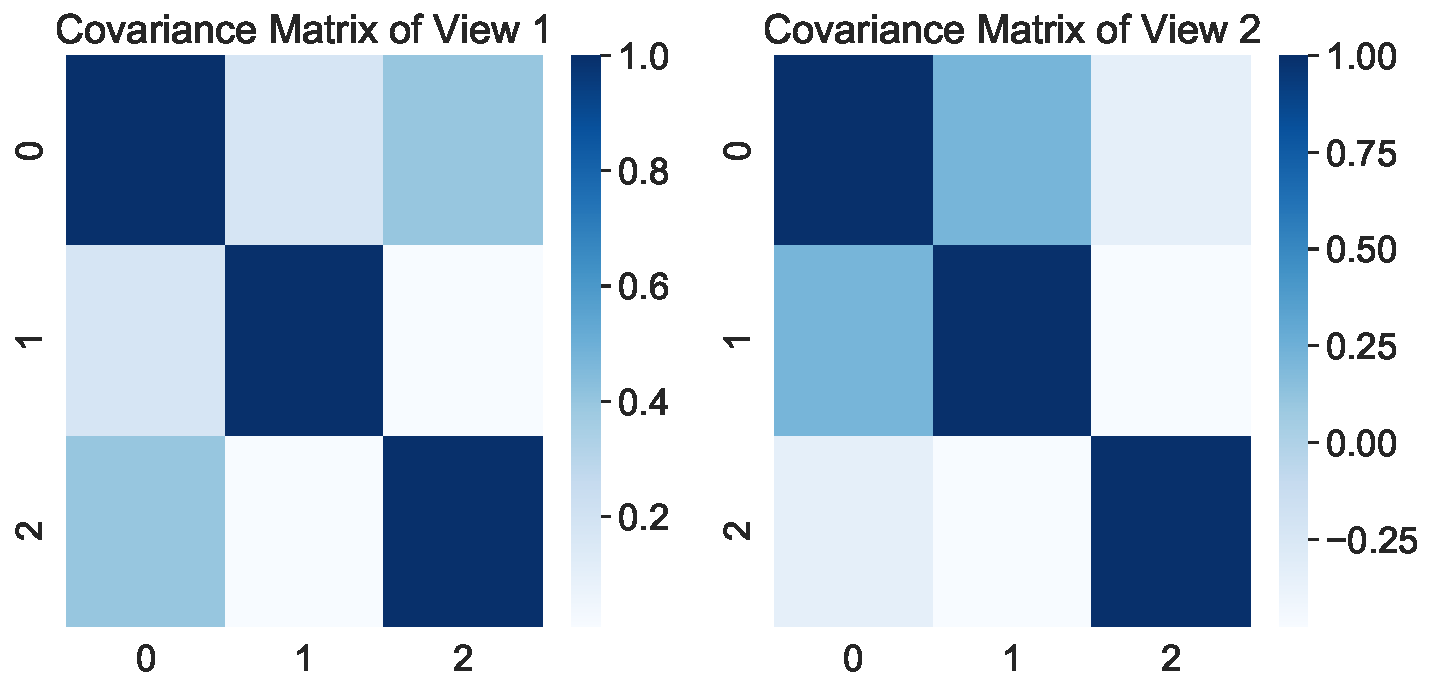
\includegraphics[width=0.8\linewidth]{figures/simulated/explicit/True_Covariance_Correlated.pdf}
     \caption{Example instances of correlated covariance matrices.}\label{fig:covariance-matrices}
 \end{figure}

Recalling table \ref{tab:covariance-structures}, note that in the implicit latent variable models, these covariance matrices are precisely the population within-view covariance matrices.
In the explicit latent variable models, these covariance matrices are just the covariance matrices of the noise to which we add the signal covariance matrices.
Nonetheless, for strong enough noise, this process ensures that there are large correlations between features.

\subsection{Assessing Information Recovery in CCA and PLS Models Under Varying Signal-to-Noise Ratios}

Our next experiment was motivated by the observation that \acrshort{pls} models (including sparse PLS) often exhibit low but non-zero out of sample correlations in real high-dimensional data.
We want to understand how much of this is due to the fact that PLS models optimize covariance rather than correlation, and how much is due to the fact that the signal-to-noise ratio is too low.
In order to understand this, we simulated data with varying signal-to-noise ratios and compared the out of sample correlations of \acrshort{pls} models with the out of sample correlations of Ridge \acrshort{cca} models with varying regularization.
We simulated data with 1000 samples and between 100 and 10,000 features in one view and 100 features in the other.
These are of the same order of magnitude as typical brain-behaviour datasets.

\paragraph{Detailed Parameters of Simulated Data for Signal-to-Noise Simulations}
We summarise these data properties in table \ref{tab:simulated-data-parameters-bb}.

\begin{table}
    \centering
    \caption{Simulated Data Parameters for Brain-Behaviour Simulations}
    \begin{tabular}{| l | l |}
        \hline
        \textbf{Parameter}                        & \textbf{Value}                               \\
        \hline
        Number of features in View 1 (\textit{p}) & 100-10000 \\
        Number of features in View 2 (\textit{q}) & 100-10000 \\
        True Latent dimensions                    & 1                                            \\
        Fraction of active features View 1            & 1.0                                          \\
        Fraction of active features View 2            & 1.0                                          \\
        Signal-to-noise ratio                    & 0.001-1 \\
        \hline
    \end{tabular}\label{tab:simulated-data-parameters-bb}
\end{table}

\section{Results of Simulations}

\subsection{Exploring the Relationship Between Weights and Loadings in CCA Using Simulated Data}

We first present the results of the experiments demonstrating the relationship between weights and \gls{loadings} in simulated data from explicit and implicit latent variable models with identity and non-identity covariance matrices.

For both cases, we plot the true weights and loadings along with the estimated weights and loadings for each model.
We estimate model loadings by multiplying the model weights by the sample within-view covariance matrix following equation \ref{eq:weights-to-loadings}.
This means that the estimated model loadings may not be sparse even when the estimated model weights are sparse and the \textit{population} covariance matrix is identity.

\subsubsection{Implicit Latent Variables (Sparse Weights)}

Figure \ref{fig:implicit-sparse-weights} shows the true and estimated weights and \gls{loadings} for data generated from the implicit latent variable models with sparse weights.
The left column shows the results for the identity covariance matrices, while the right column shows the results for the correlated covariance matrices.
Figure \ref{fig:implicit-test-correlations} shows the test correlations for the models.

\textcolor{red}{TO-DO: Interpret these results. Key thing, CCA best performing under identity noise covariance, but Ridge CCA best performing under correlated covariance. Loadings of CCA and Ridge CCA are much more similar across models than weights.}

% %Weights/Loadings
% \begin{figure}
% \centering
% \begin{subfigure}{0.49\linewidth}
% \centering
% 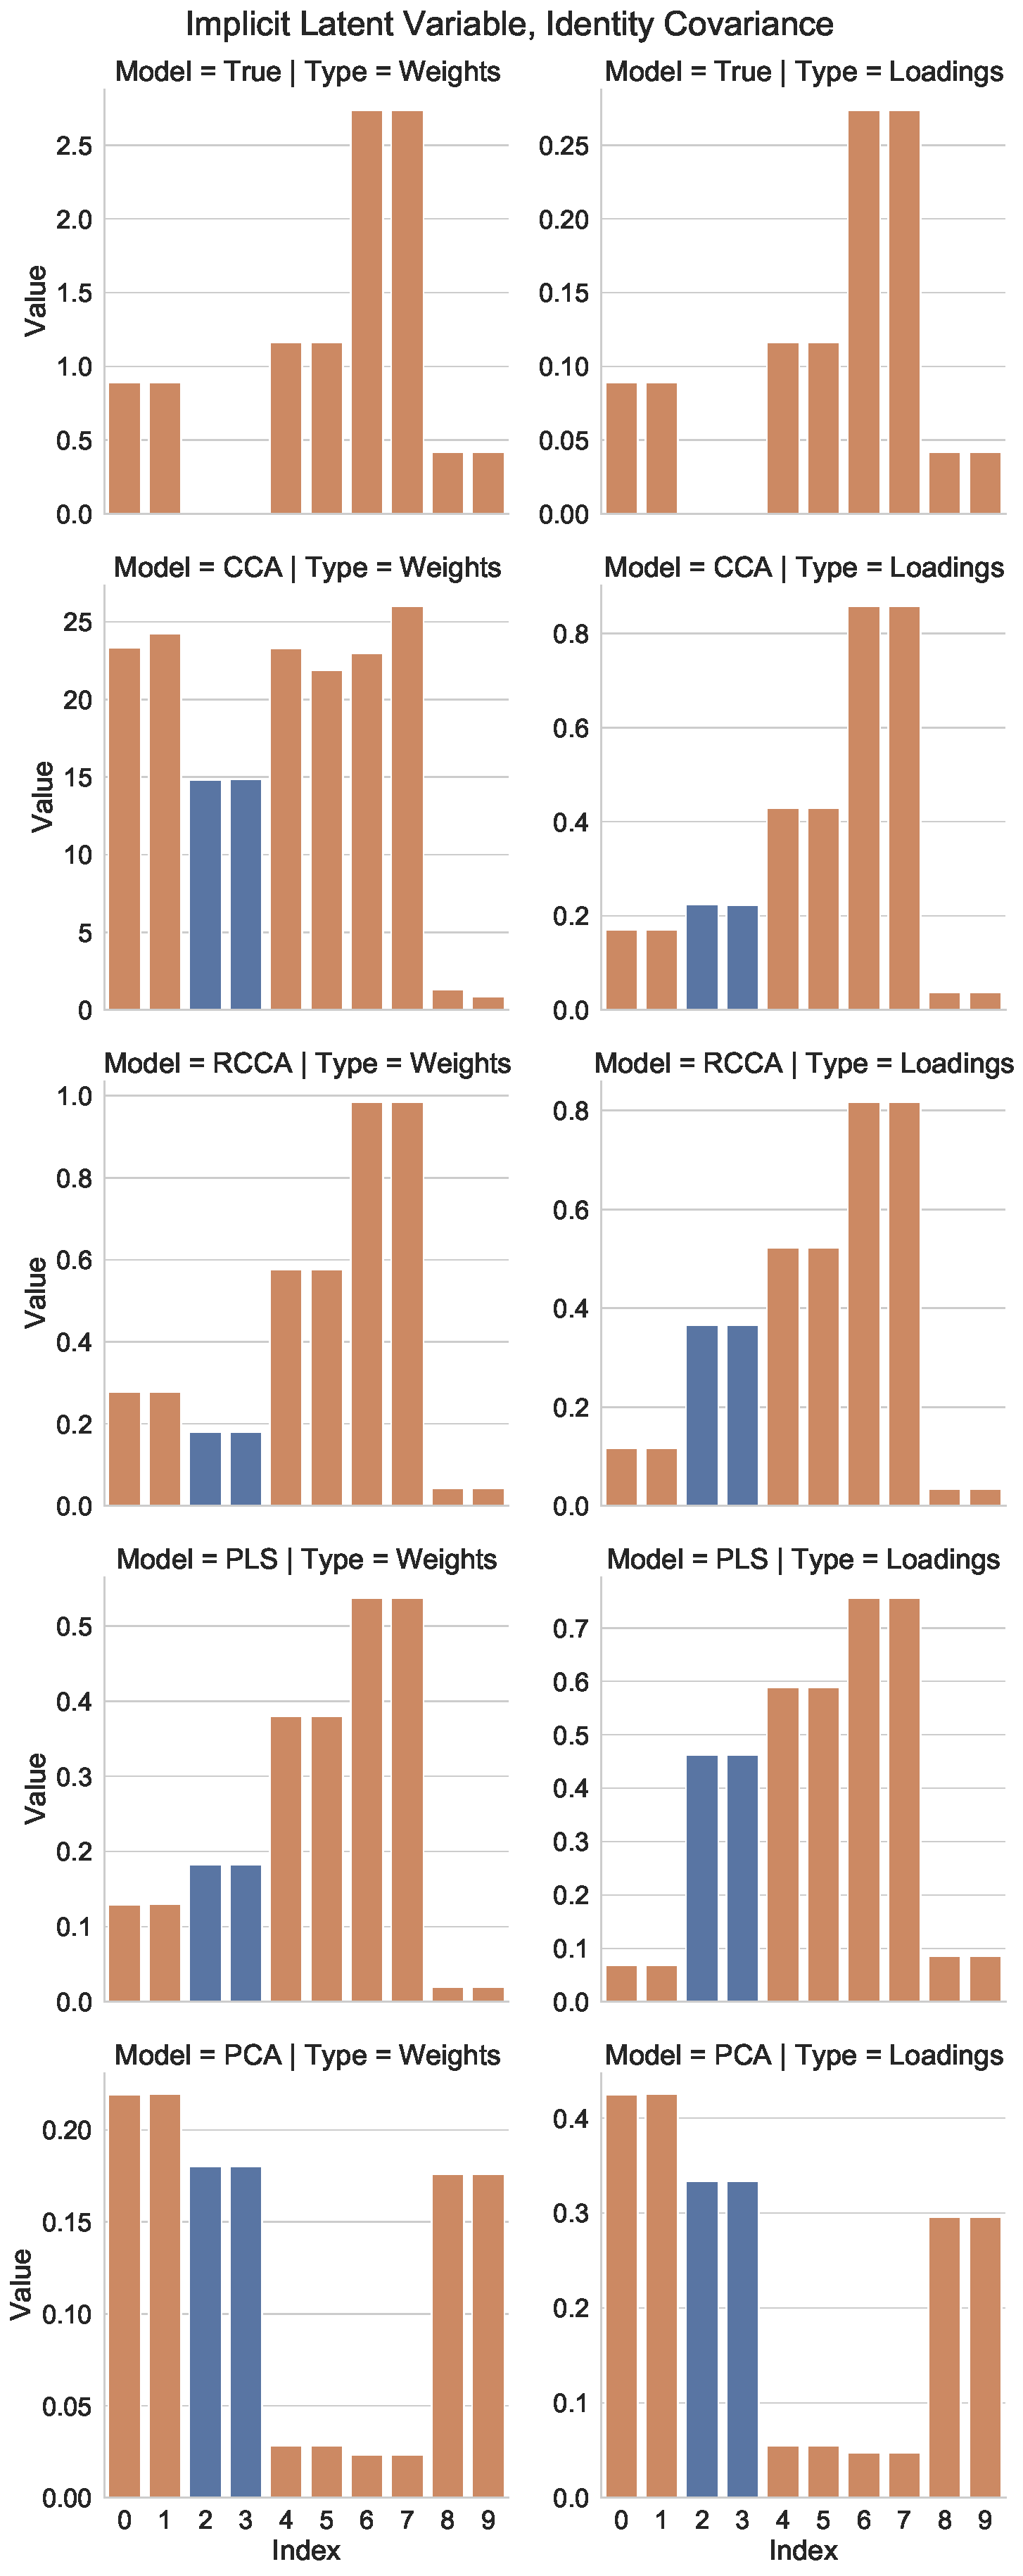
\includegraphics[width=\linewidth]{figures/simulated/Combined_Weights_Loadings_with_Error_Bars_Identity_Covariance_implicit.pdf}
% \end{subfigure}
% %
% \begin{subfigure}{0.49\linewidth}
% \centering
% 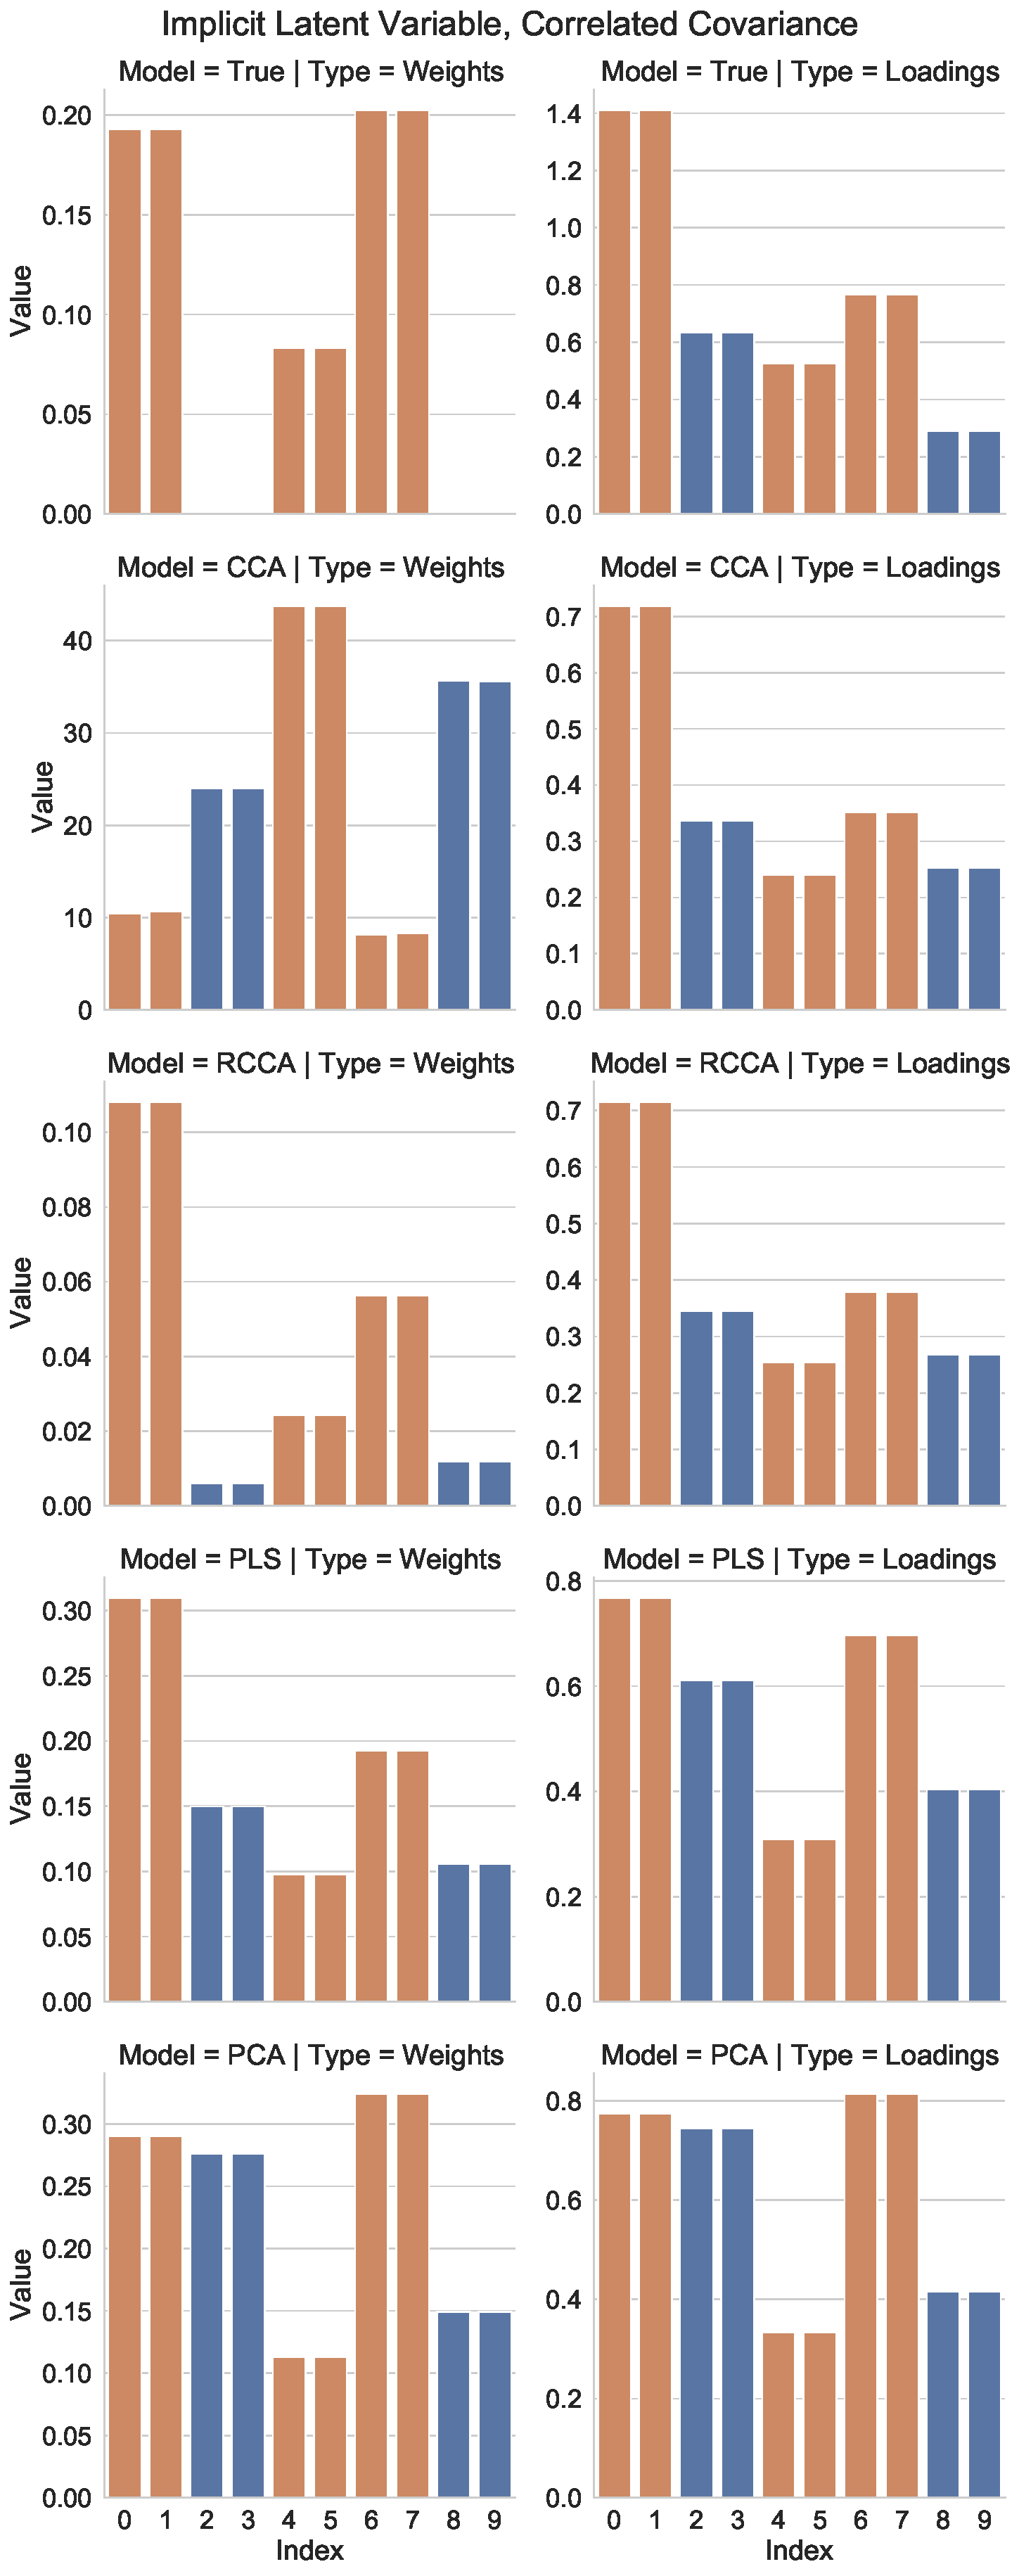
\includegraphics[width=\linewidth]{figures/simulated/Combined_Weights_Loadings_with_Error_Bars_Correlated_Covariance_implicit.pdf}
% \end{subfigure}
%     \caption{Implicit Latent Variables (Sparse Weights)}\label{fig:implicit-sparse-weights}
% \end{figure}

% %Correlation
% \begin{figure}
%     \centering
%     \begin{subfigure}{0.49\linewidth}
%         \centering
%         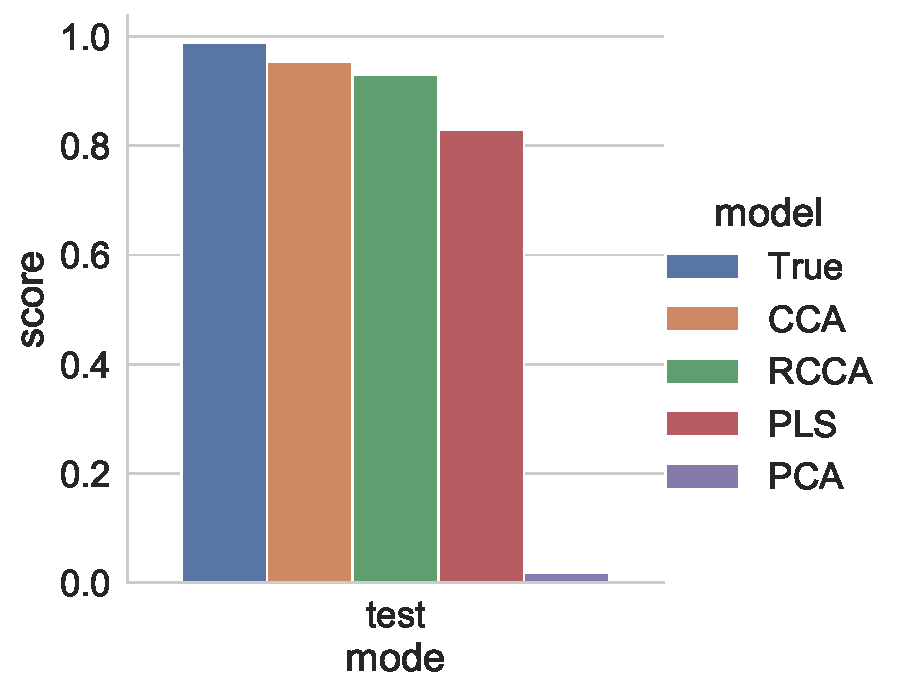
\includegraphics[width=\linewidth]{figures/simulated/Train_Test_Scores_Identity_Covariance_implicit.pdf}
%         \caption{Identity Covariance}
%     \end{subfigure}
% %
%     \begin{subfigure}{0.49\linewidth}
%         \centering
%         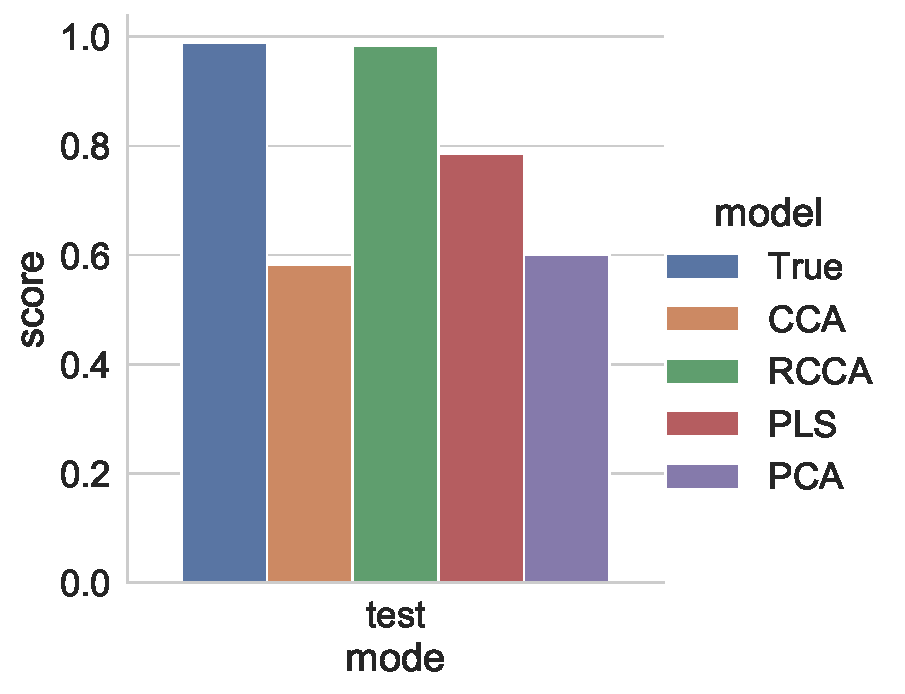
\includegraphics[width=\linewidth]{figures/simulated/Train_Test_Scores_Correlated_Covariance_implicit.pdf}
%         \caption{Correlated Covariance}
%     \end{subfigure}
%     \caption{Explicit Latent Variables: Test Correlations}\label{fig:implicit-test-correlations}
% \end{figure}

\subsubsection{Explicit Latent Variables (Sparse Weights)}

Figure \ref{fig:explicit-sparse-loadings} shows the true and estimated weights and \gls{loadings} for data generated from the explicit latent variable models with sparse \gls{loadings}.
The left column shows the results for the identity covariance matrices, while the right column shows the results for the correlated covariance matrices.
Figure \ref{fig:explicit-test-correlations} shows the test correlations for the models.

\textcolor{red}{TO-DO: Interpret these results. Key thing, under identity noise covariance, even PCA performs well as does PLS. }

% \begin{figure}
% \centering
% \begin{subfigure}{0.49\linewidth}
% \centering
% 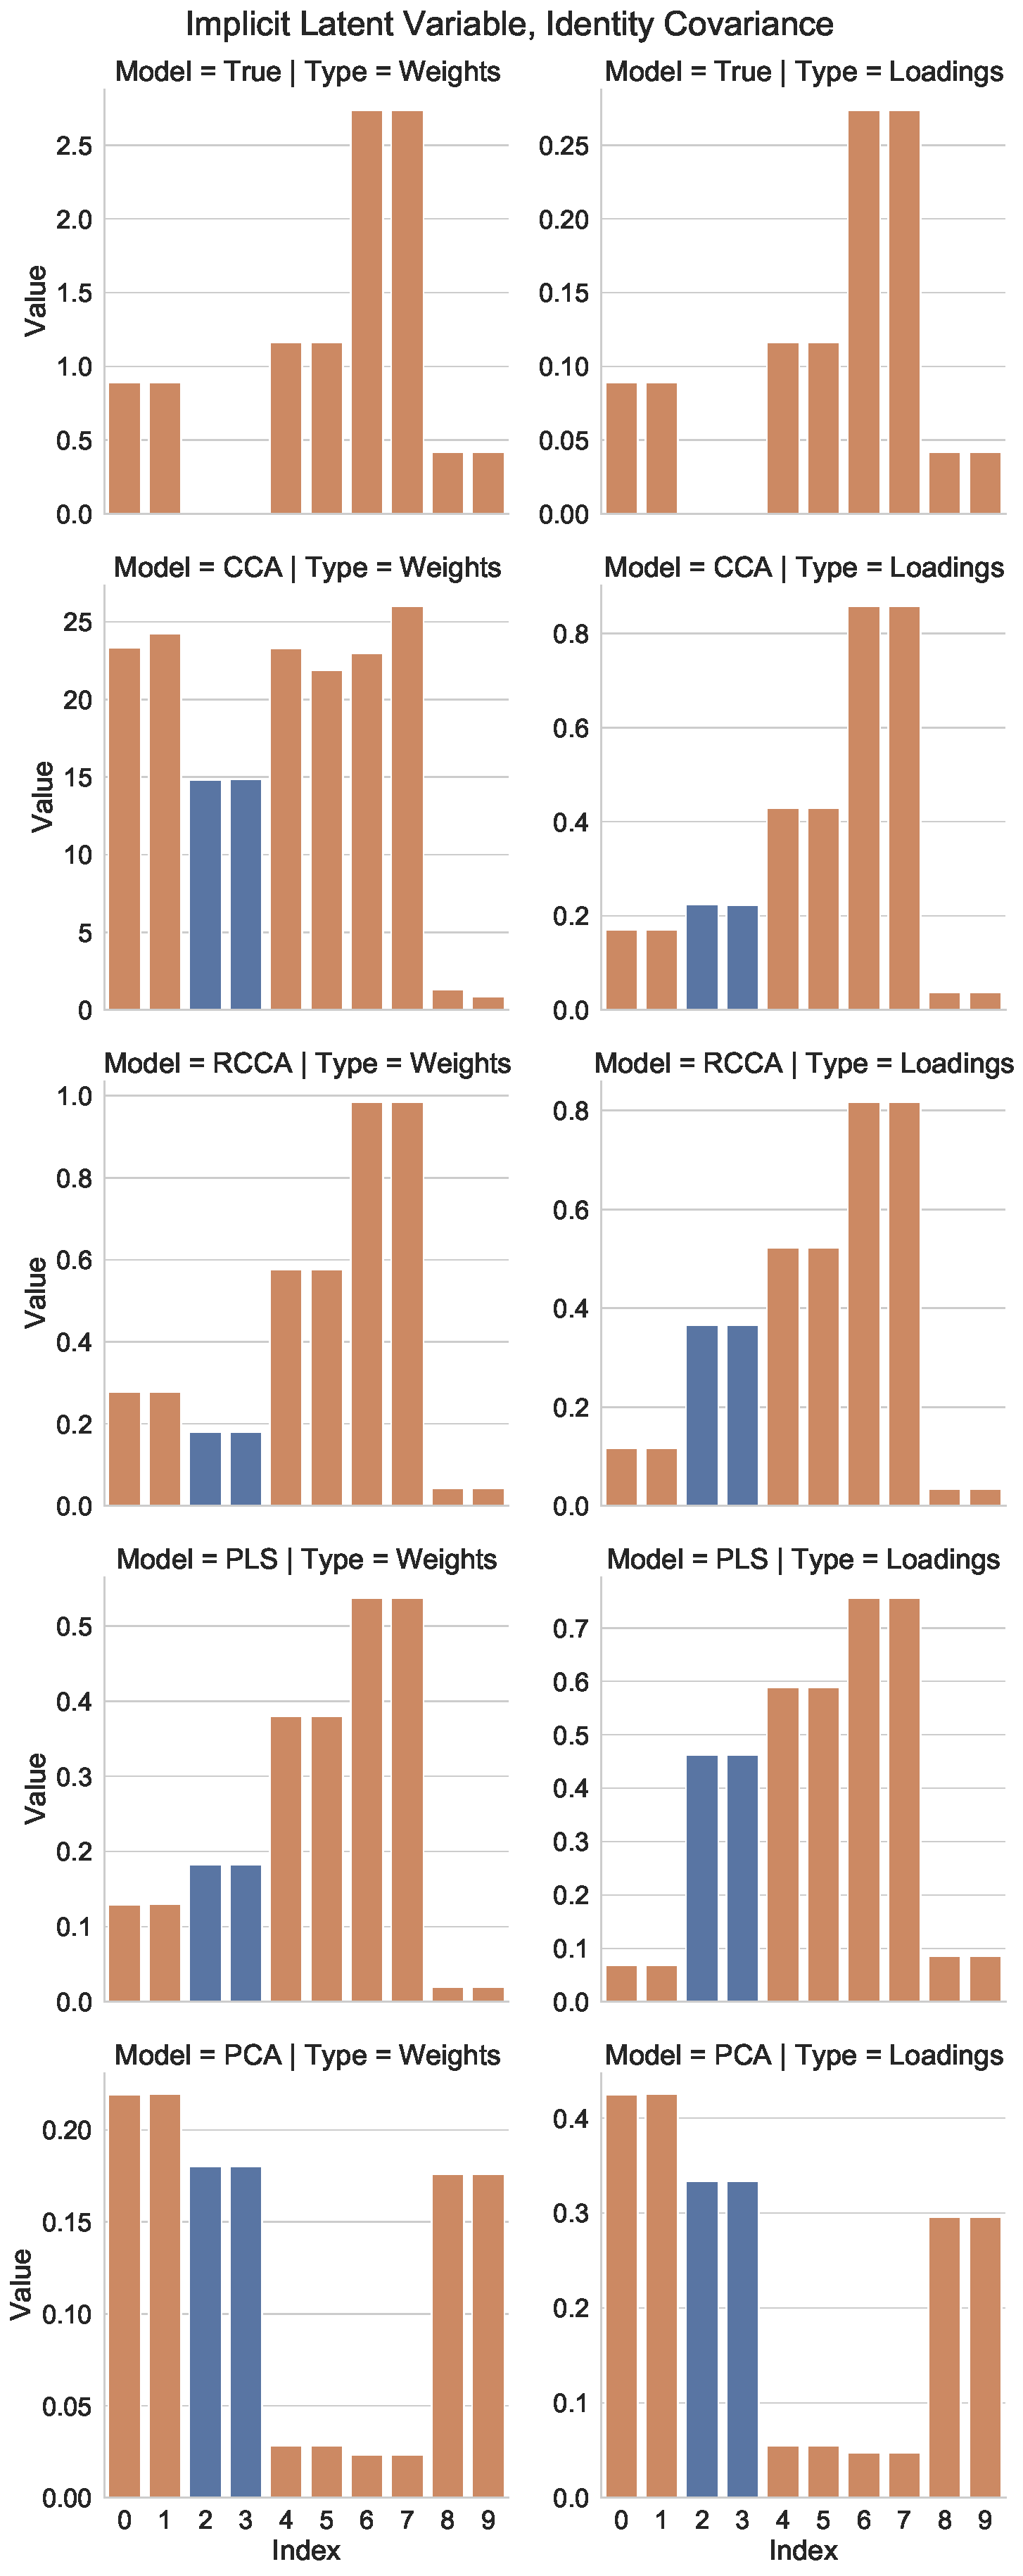
\includegraphics[width=\linewidth]{figures/simulated/Combined_Weights_Loadings_with_Error_Bars_Identity_Covariance_implicit.pdf}
% \end{subfigure}
% %
% \begin{subfigure}{0.49\linewidth}
% \centering
% 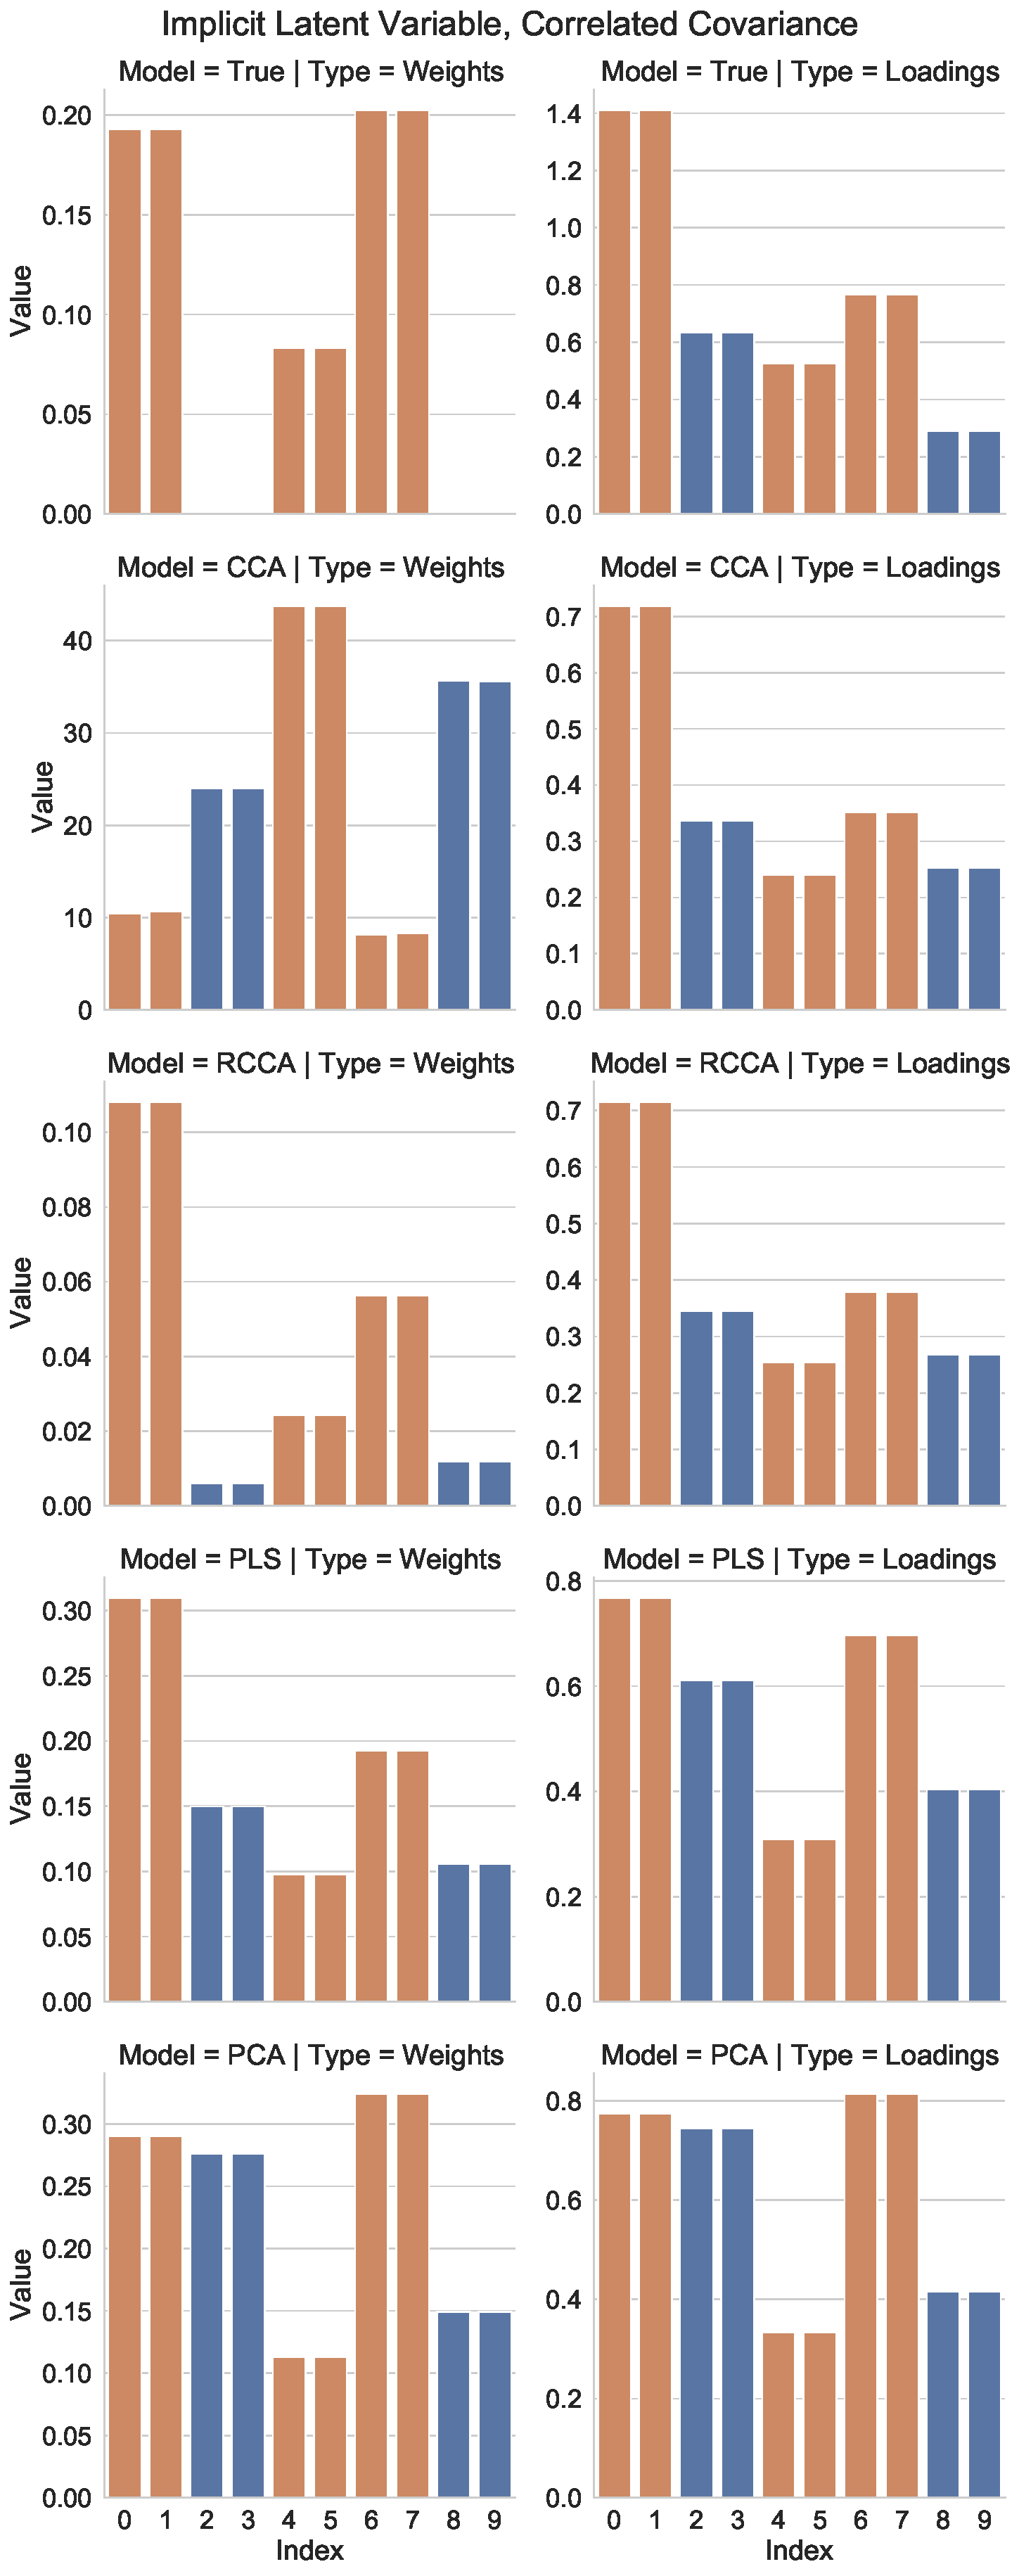
\includegraphics[width=\linewidth]{figures/simulated/Combined_Weights_Loadings_with_Error_Bars_Correlated_Covariance_implicit.pdf}
% \end{subfigure}
%     \caption{Explicit Latent Variables (Sparse Loadings)}\label{fig:explicit-sparse-loadings}
% \end{figure}

% %Correlation
% \begin{figure}
%     \centering
%     \begin{subfigure}{0.49\linewidth}
%         \centering
%         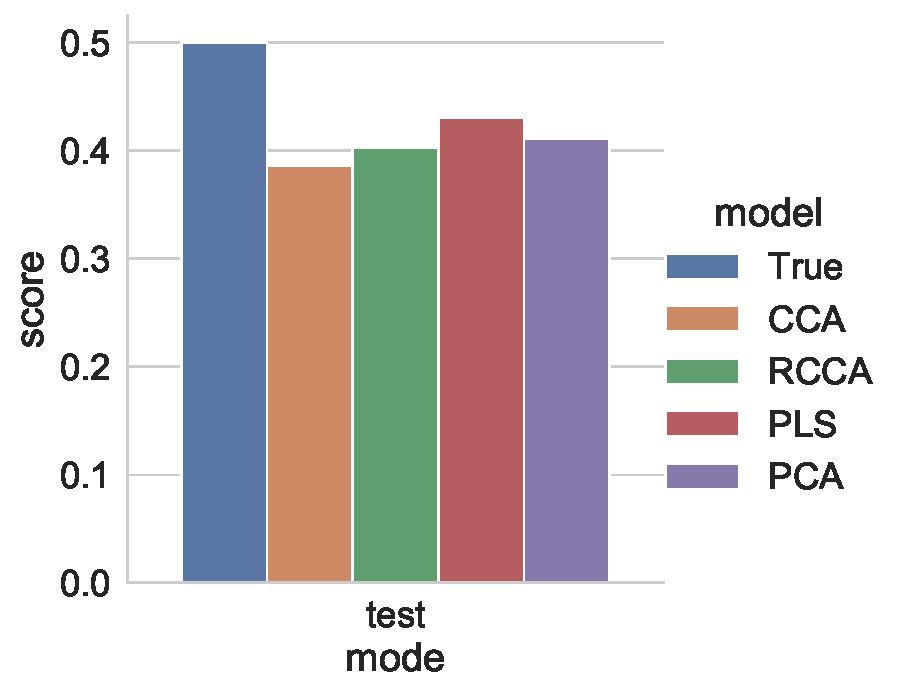
\includegraphics[width=\linewidth]{figures/simulated/Train_Test_Scores_Identity_Covariance_explicit.pdf}
%         \caption{Identity Covariance}
%     \end{subfigure}
% %
%     \begin{subfigure}{0.49\linewidth}
%         \centering
%         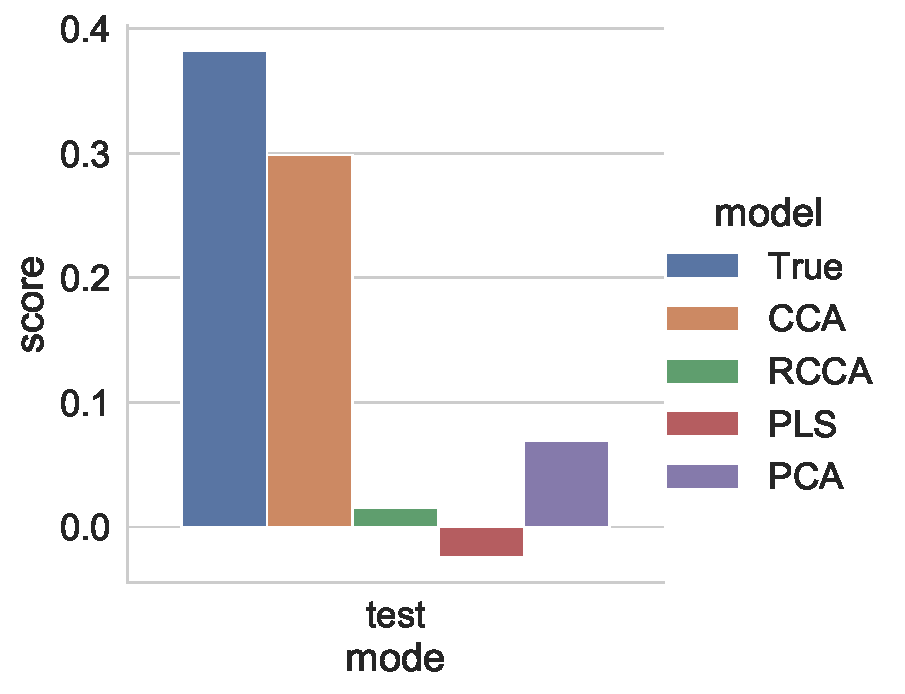
\includegraphics[width=\linewidth]{figures/simulated/Train_Test_Scores_Correlated_Covariance_explicit.pdf}
%         \caption{Correlated Covariance}
%     \end{subfigure}
%     \caption{Explicit Latent Variables: Test Correlations}
% \end{figure}

\subsubsection{Measuring the Identitiness of the Covariance Matrices}
The theory we developed in section~\ref{sec:generative-perspectives} suggests that the closer to identity the covariance matrices are, the closer the weights and \gls{loadings} will be.
This is particularly important if we want to use structure inducing regularisation of the backward model (such as FRALS framework from chapter \ref{ch:als}) as the structural priors (e.g. sparsity) will only translate to equivalent structural priors the forward model if the covariance matrices are close to identity.
We develop a simple graphical way to compare the identitiness of the covariance matrices by plotting the eigenvalues of the covariance matrices.
If the eigenvalues of the sample covariance matrix are all close to 1, then the sample covariance matrix is close to identity.
Departures from 1 indicate that the sample covariance matrix is not close to identity and imply multicollinearity in the data.

In the simulated data, we can see that the data generation models with identity noise covariance matrices, have eigenvalues closer to one than (Figure~\ref{fig:covariance-eigenvalues-simulated-low}).
On the other hand, these plots show that all the \textit{sample} covariance matrices depart from the ideal case, even when the \textit{population} covariance matrices are precisely identity.

\begin{figure}
    \centering
    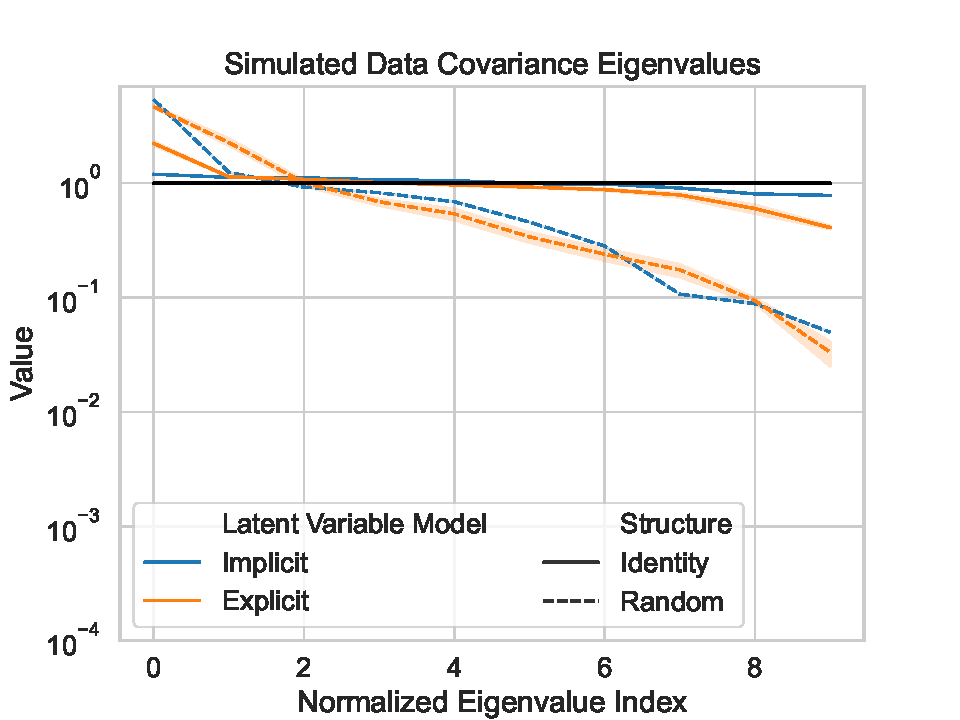
\includegraphics[width=0.8\linewidth]{figures/covariance/simulated_covariance_eigenvalues_low}
    \caption{Eigenvalues of the covariance matrices for the simulated datasets.}\label{fig:covariance-eigenvalues-simulated-low}
\end{figure}


\subsection{Assessing Information Recovery in CCA and PLS Models Under Varying Signal-to-Noise Ratios}

In Figures \ref{fig:snr-scores-identity} and \ref{fig:snr-scores-random} we plot the test correlation (score) varying the signal-to-noise ratio and the number of features.

\textcolor{red}{TO-DO: Interpret these results. Key idea, under identity noise covariance, PLS is fine for modelling correlation and so are ridge regularized CCA models. Under random noise covariance, PLS is not fine and is vastly outperformed by ridge regularized CCA models. This is because PLS is optimizing covariance not correlation.})

\begin{figure}
    \centering
    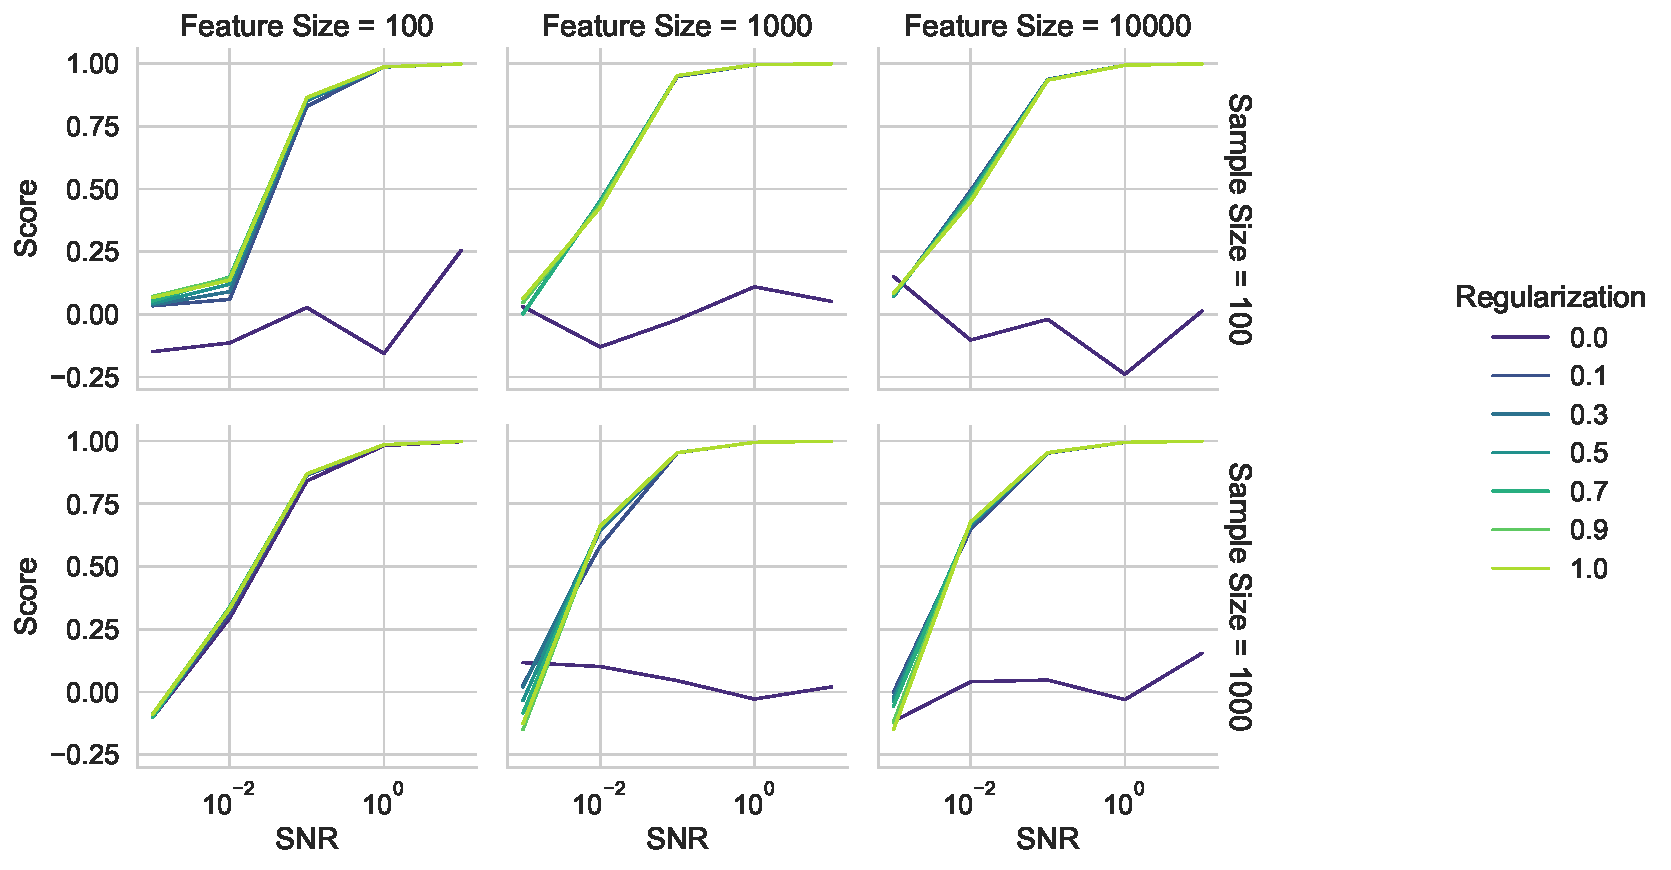
\includegraphics[width=\linewidth]{figures/brain_behaviour_sim/snr_vs_scores_facet_identity}
    \caption{Varying signal to noise ratio with identity covariance matrices}\label{fig:snr-scores-identity}
\end{figure}

\begin{figure}
    \centering
    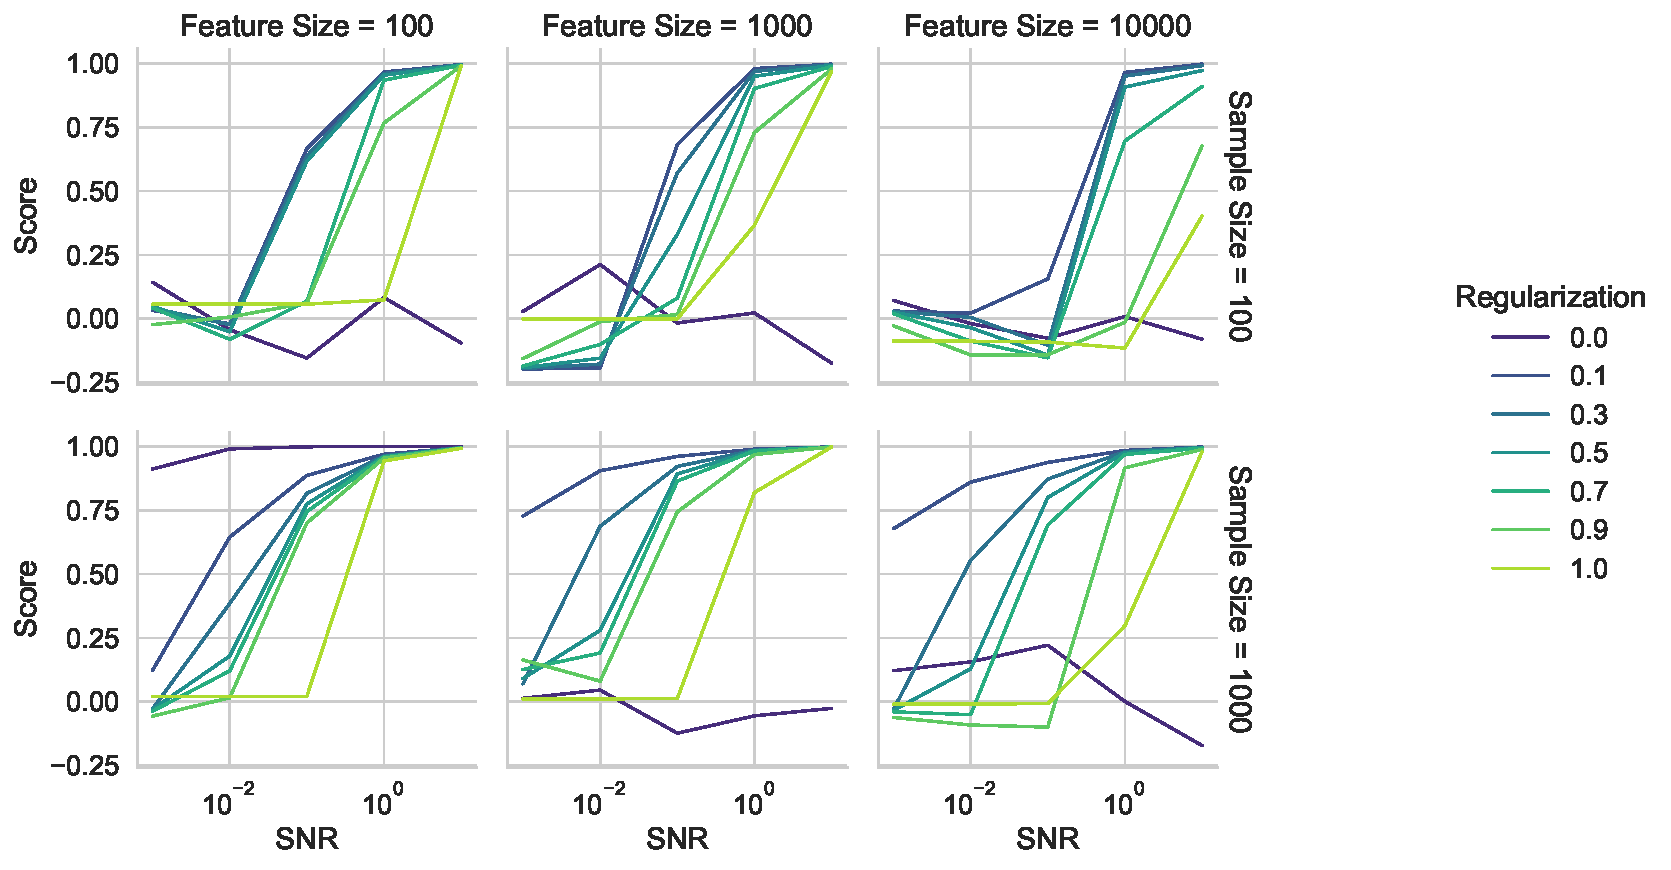
\includegraphics[width=\linewidth]{figures/brain_behaviour_sim/snr_vs_scores_facet_random}
    \caption{arying signal to noise ratio with correlated covariance matrices}\label{fig:snr-scores-random}
\end{figure}

\section{Revisiting Brain-Behaviour Results}



In this section, we revisit the results from the brain-behaviour experiments in Chapter \ref{ch:als} by comparing the weights and \gls{loadings} of the \acrshort{hcp} and \acrshort{adni} datasets.

\textcolor{red}{TO-DO: Revisit FRALS experiments through the lens of loadings.}

\subsection{Identitiness of Covariance Matrices}
In this section, we consider the identitiness of the covariance matrices for the \acrshort{hcp} and \acrshort{adni} datasets.
Figure \ref{fig:covariance-eigenvalues-real} shows the eigenvalues of the covariance matrices for the \acrshort{hcp} and \acrshort{adni} datasets while Figure \ref{fig:covariance-matrices-real} shows the covariance matrices themselves (with the \acrshort{adni} brain covariance matrix left out due to its size).
From Figure \ref{fig:covariance-eigenvalues-real}, we can see that the eigenvalues of the covariance matrices for the \acrshort{adni} data are much closer to the ideal for identity covariance than for the \acrshort{hcp} data.
\begin{figure}
    \centering
    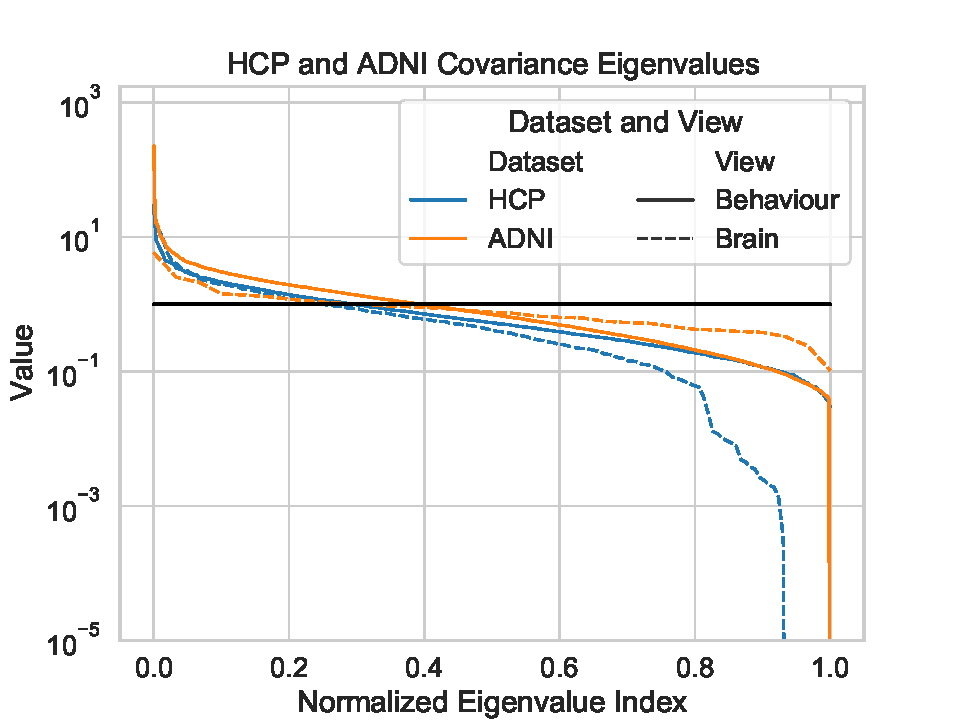
\includegraphics[width=0.8\linewidth]{figures/covariance/hcp_adni_covariance_eigenvalues}
    \caption{Eigenvalues of the covariance matrices for the \acrshort{hcp} and \acrshort{adni} datasets.}\label{fig:covariance-eigenvalues-real}
\end{figure}
%
%From Figure \ref{fig:covariance-matrices-real}, we can see the block structure of the covariance matrices.
%
%\begin{figure}
%    \centering
%    \begin{subfigure}{0.66\linewidth}
%        \centering
%        \includegraphics[width=\linewidth]{figures/covariance/hcp_covariance}
%        \caption{\acrshort{hcp}}
%    \end{subfigure}
%%
%    \begin{subfigure}{0.33\linewidth}
%        \centering
%        \includegraphics[width=\linewidth]{figures/covariance/adni_covariance}
%        \caption{\acrshort{adni}}
%    \end{subfigure}
%    \caption{Covariance matrices for the \acrshort{hcp} and \acrshort{adni} datasets.}
%    \label{fig:covariance-matrices-real}
%\end{figure}
%
%\subsection{Loading Similarity}
%
%`\begin{figure}
%     \centering
%     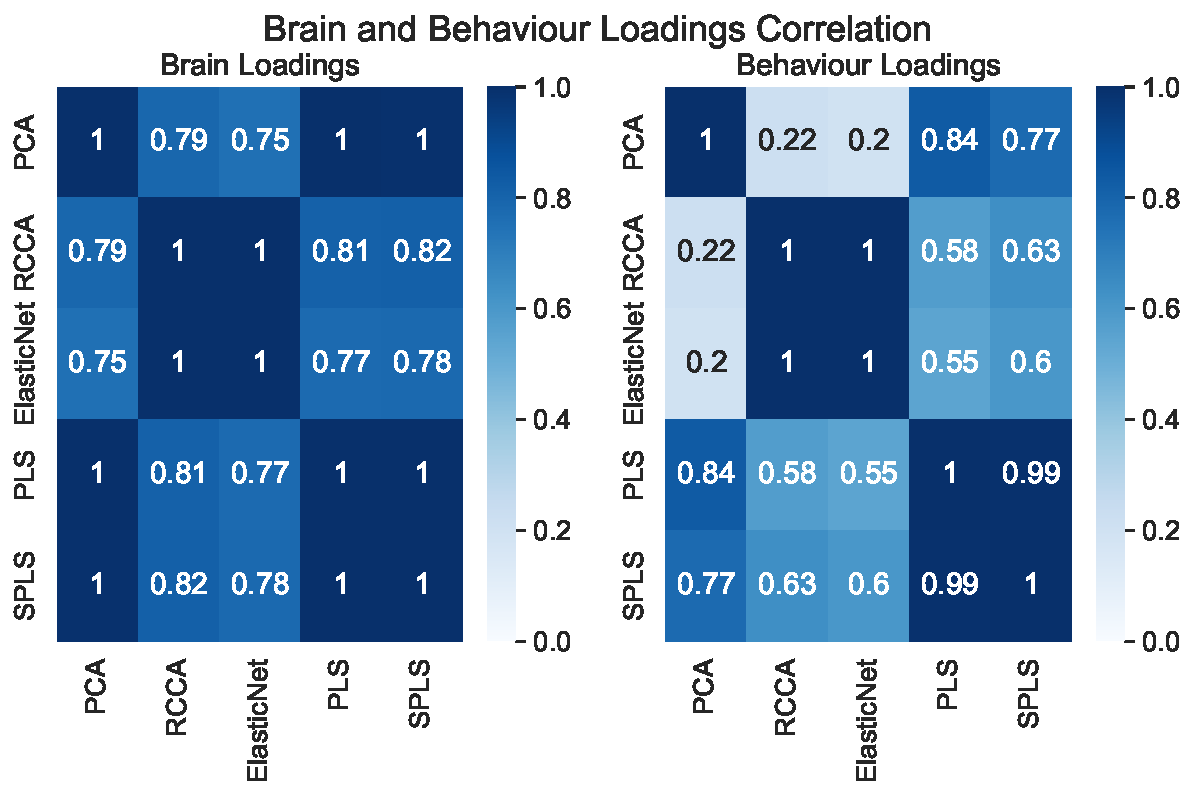
\includegraphics[width=0.8\linewidth]{figures/hcp/brain and behaviour loadings correlation}
%     \caption{\textbf{HCP:} Correlation between the brain and behaviour \gls{representations} for each model.}
%\end{figure}
%
%\begin{figure}
%    \centering
%    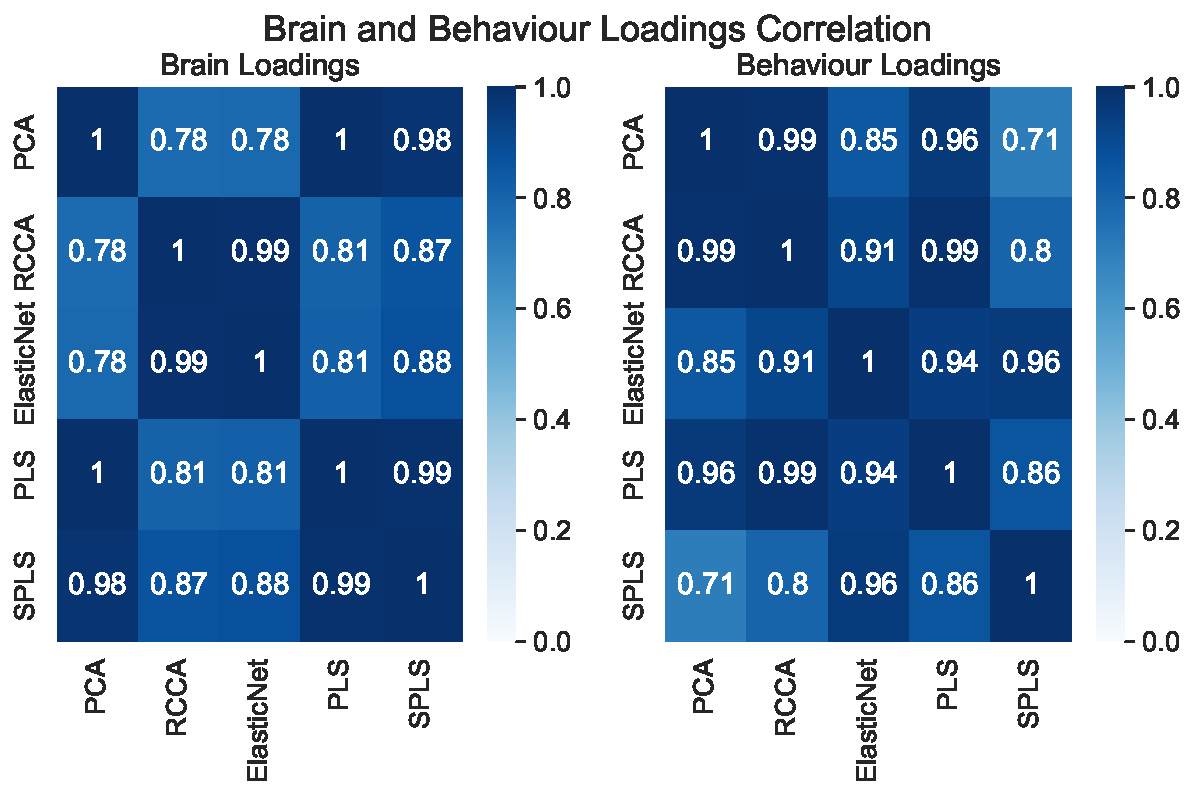
\includegraphics[width=0.8\linewidth]{figures/adni/brain and behaviour loadings correlation}
%    \caption{\textbf{ADNI:} Correlation between the brain and behaviour \gls{representations} for each model.}
%\end{figure}
%
%\subsection{Comparing Behaviour Weights and Loadings}
%
%\subsubsection{Human Connectome Project (\acrshort{hcp}) Data}
%
%\begin{figure}
%    \centering
%    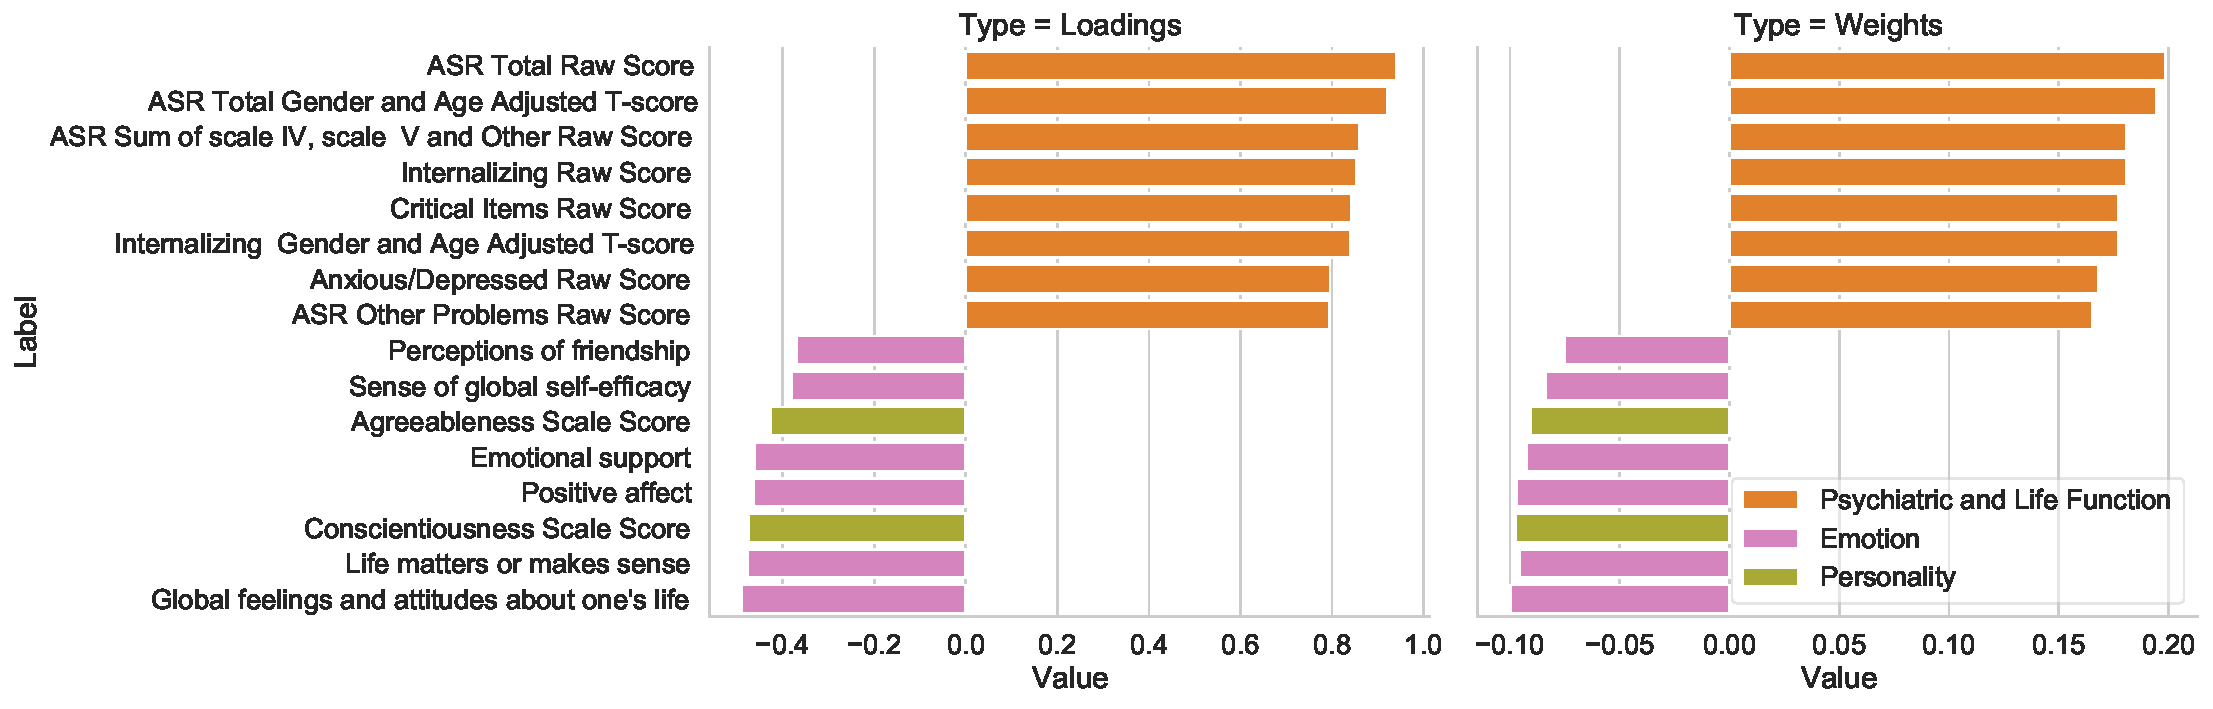
\includegraphics[width=0.8\linewidth]{figures/hcp/PCA behaviour weights and loadings}
%    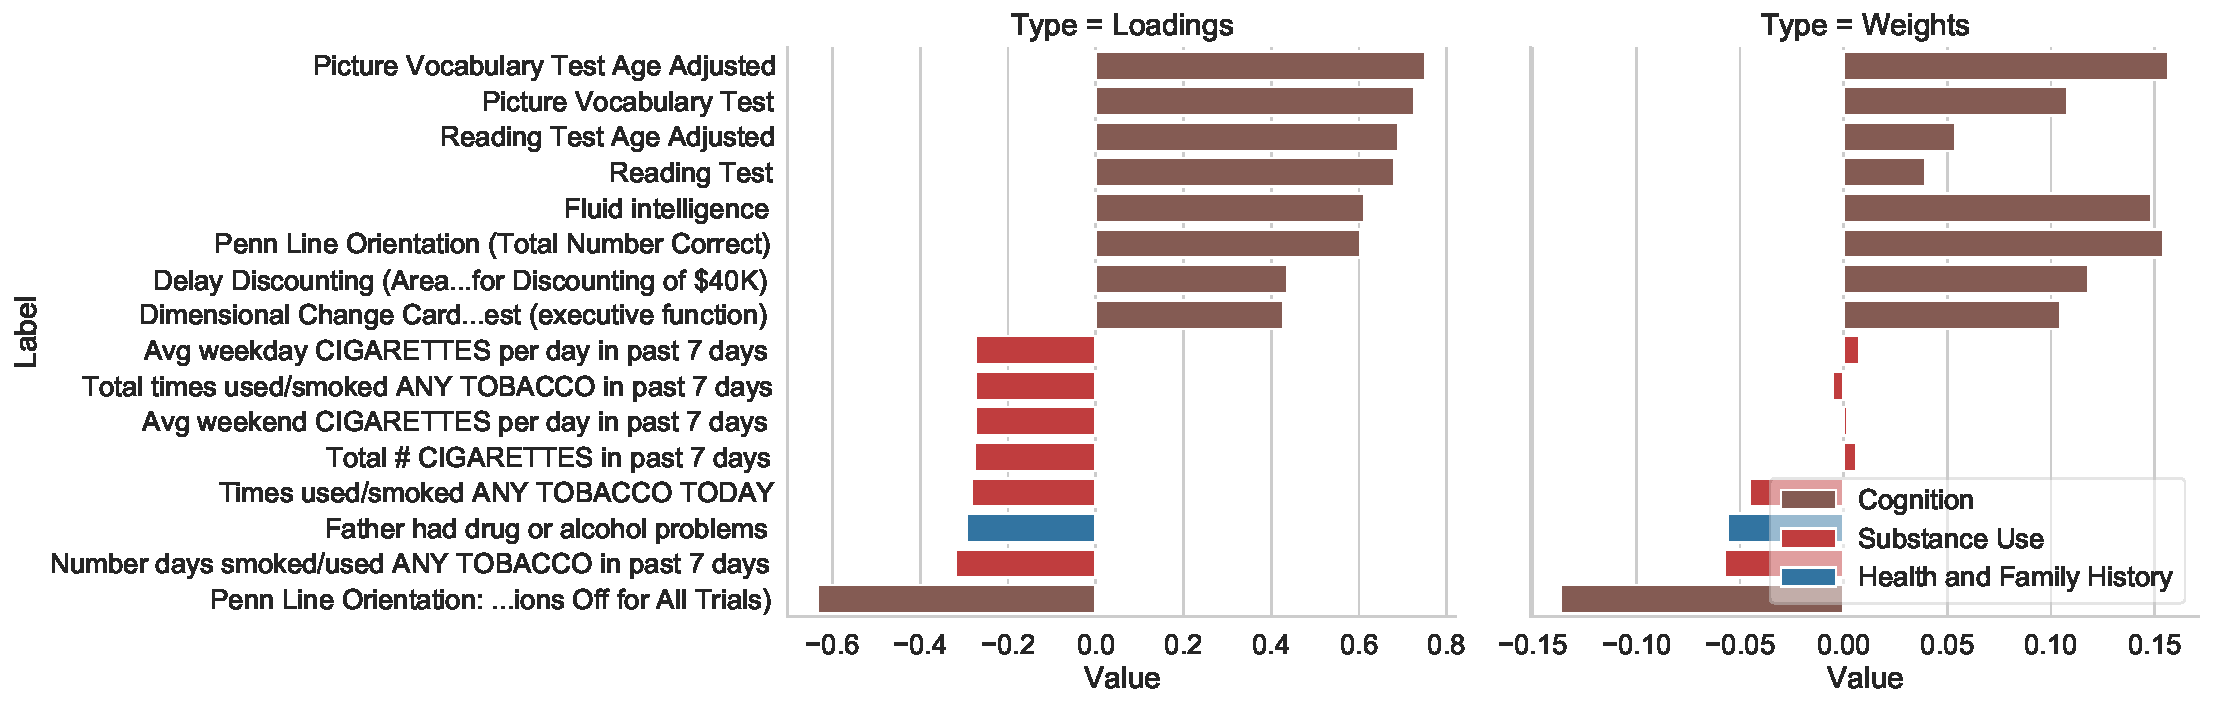
\includegraphics[width=0.8\linewidth]{figures/hcp/RCCA behaviour weights and loadings}
%    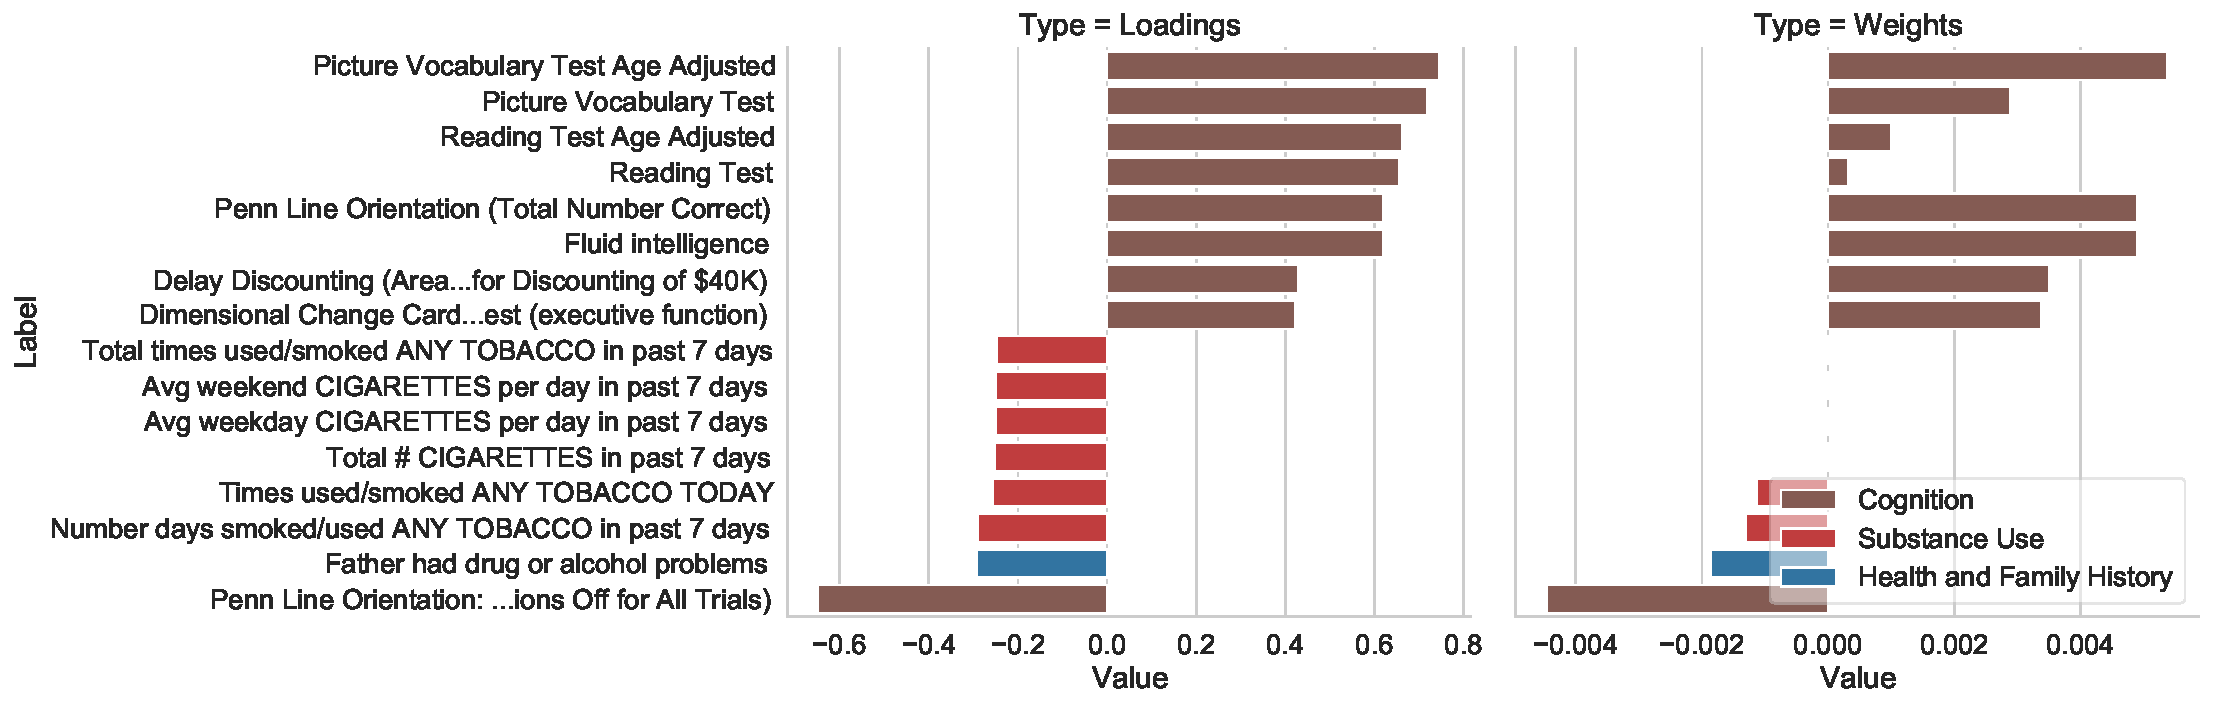
\includegraphics[width=0.8\linewidth]{figures/hcp/ElasticNet behaviour weights and loadings}
%    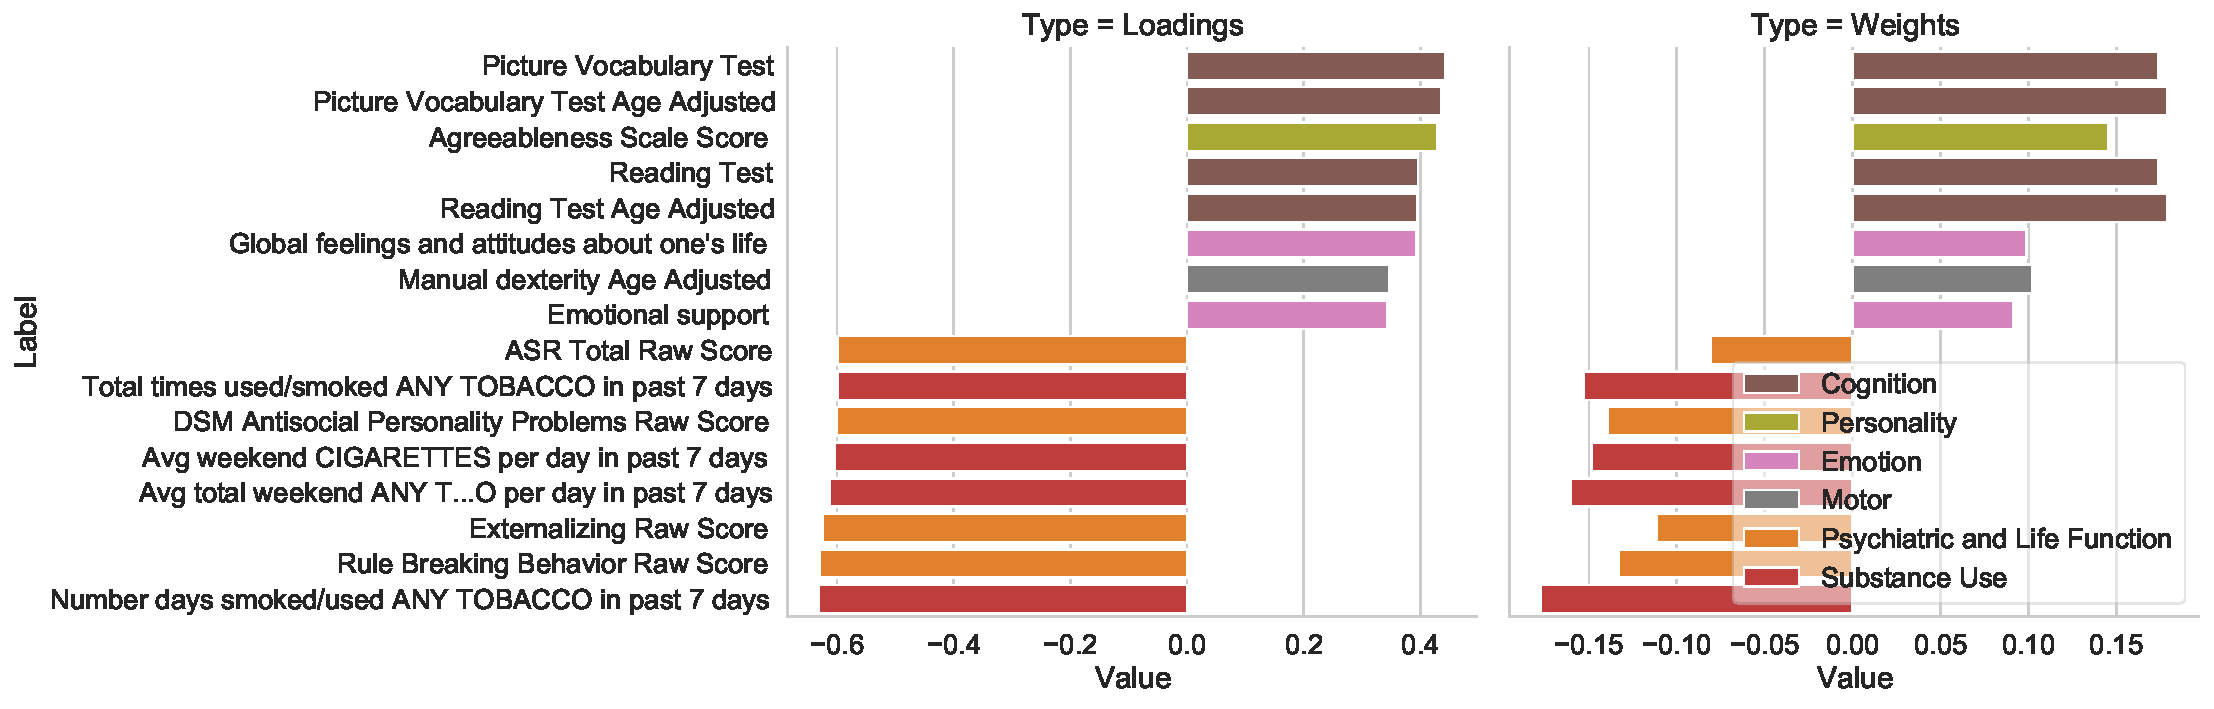
\includegraphics[width=0.8\linewidth]{figures/hcp/PLS behaviour weights and loadings}
%    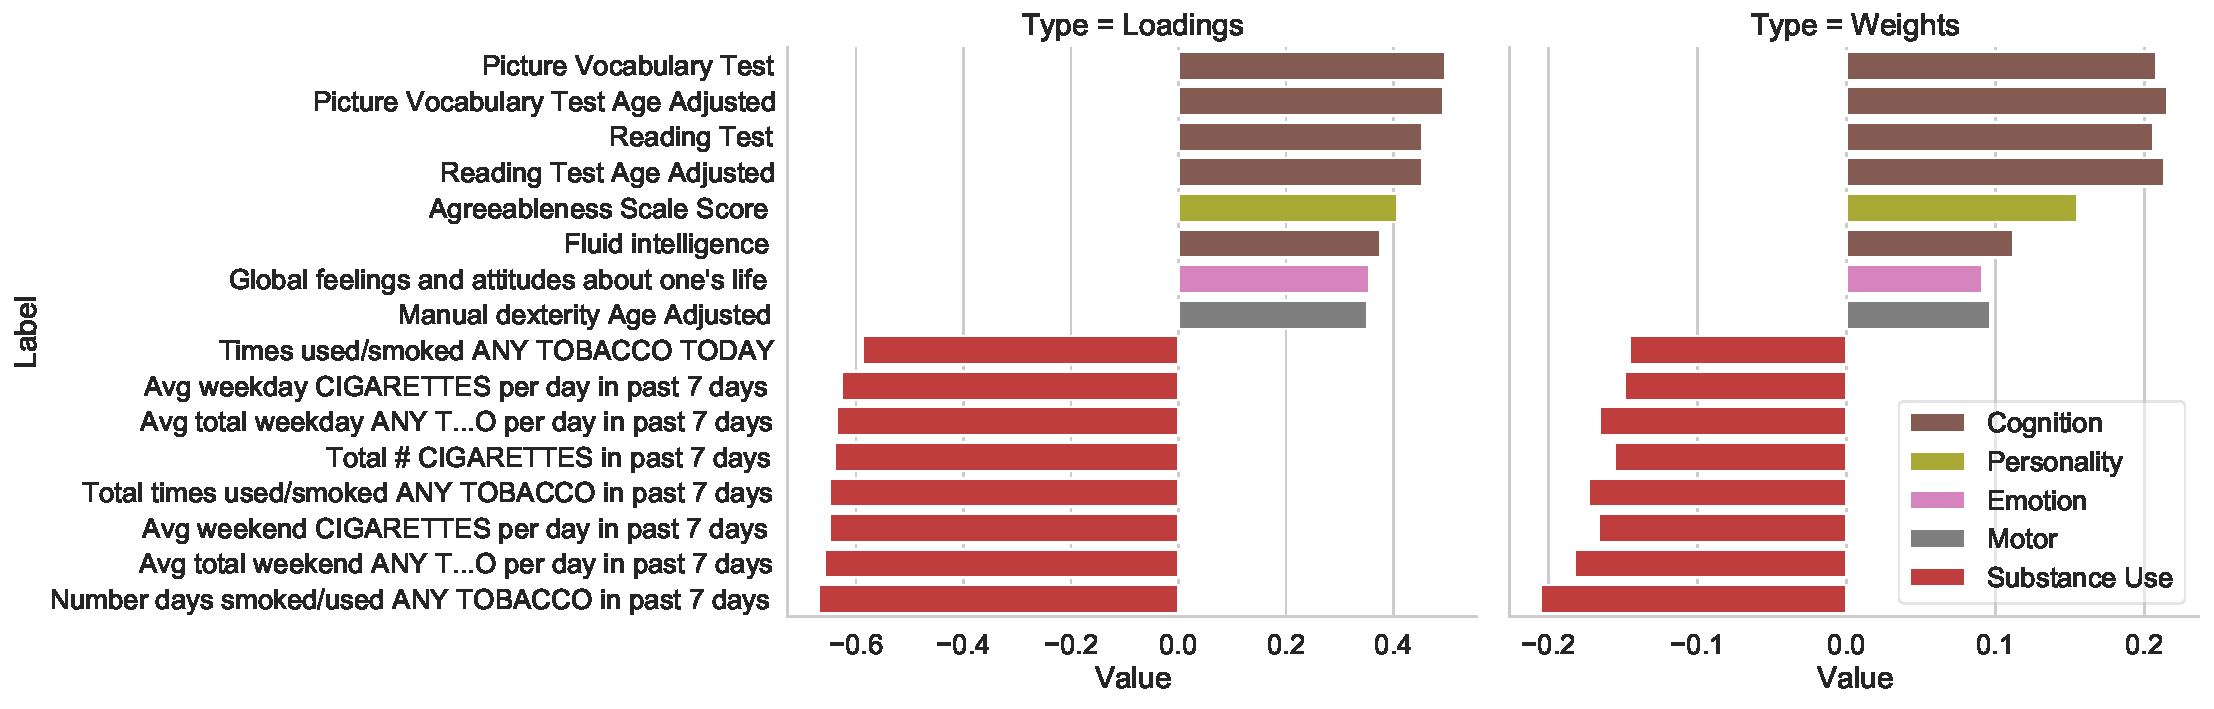
\includegraphics[width=0.8\linewidth]{figures/hcp/SPLS behaviour weights and loadings}
%    \caption{Top 8 positive and negative non-imaging \gls{loadings} for each model}
%\end{figure}
%
%\subsubsection{Alzheimer's Disease Neuroimaging Initiative (\acrshort{adni}) Data}
%
%\begin{figure}
%    \centering
%    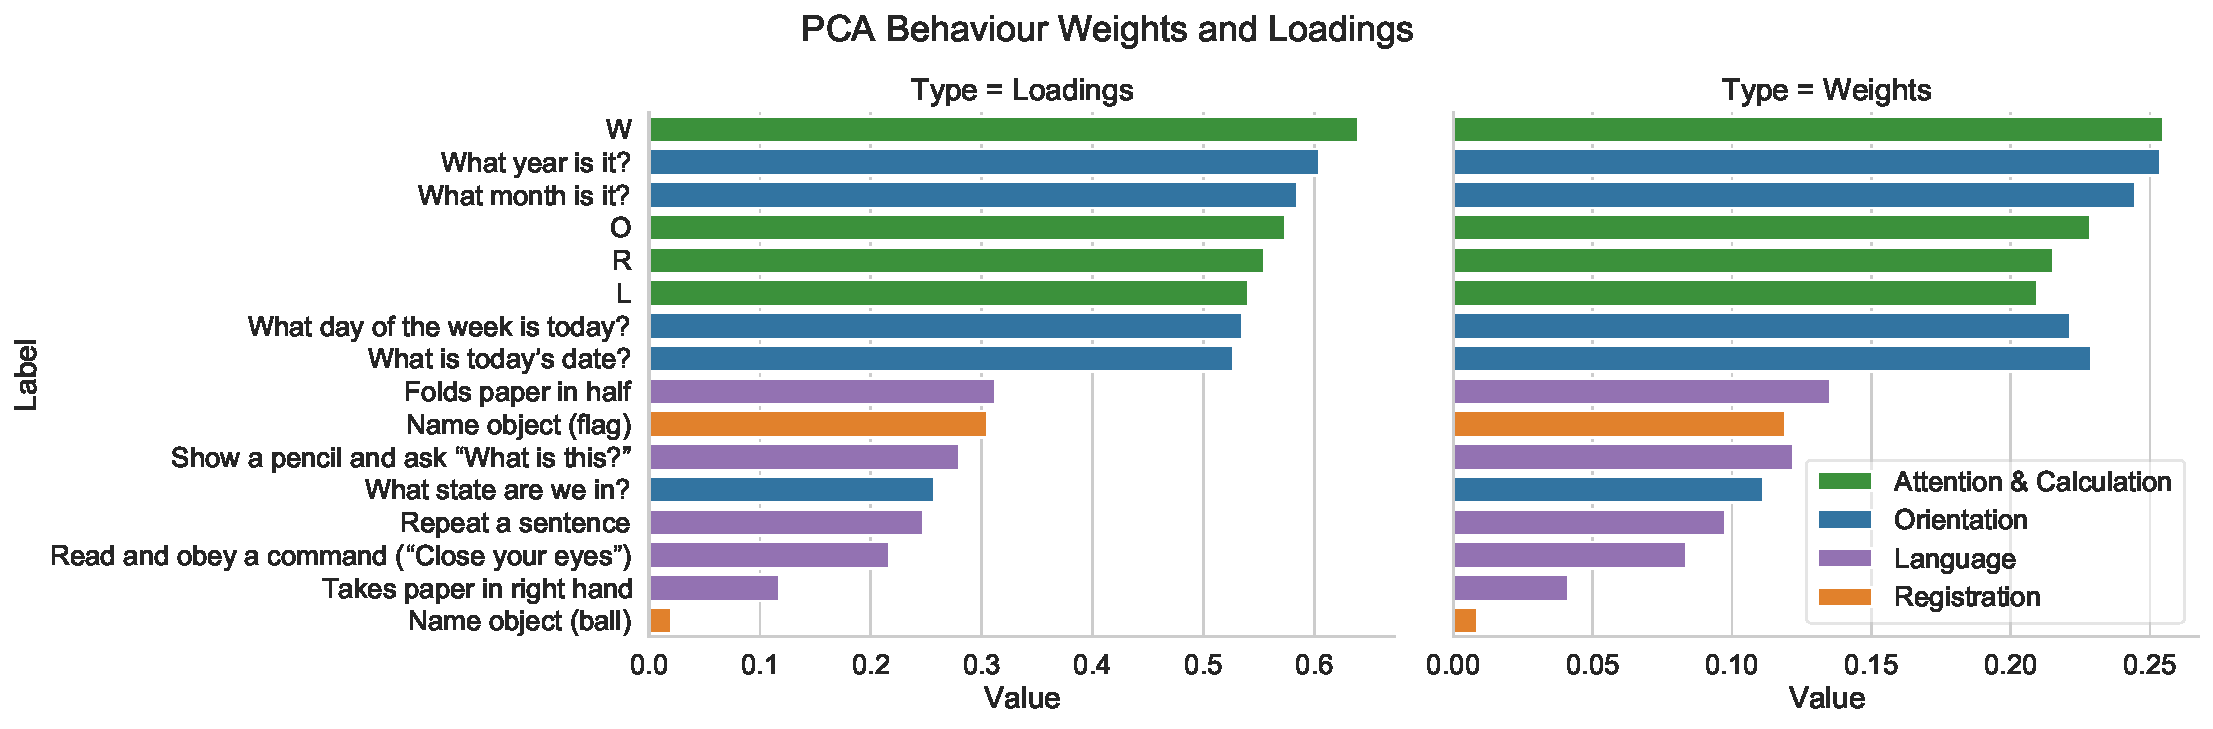
\includegraphics[width=0.8\linewidth]{figures/adni/PCA behaviour weights and loadings}
%    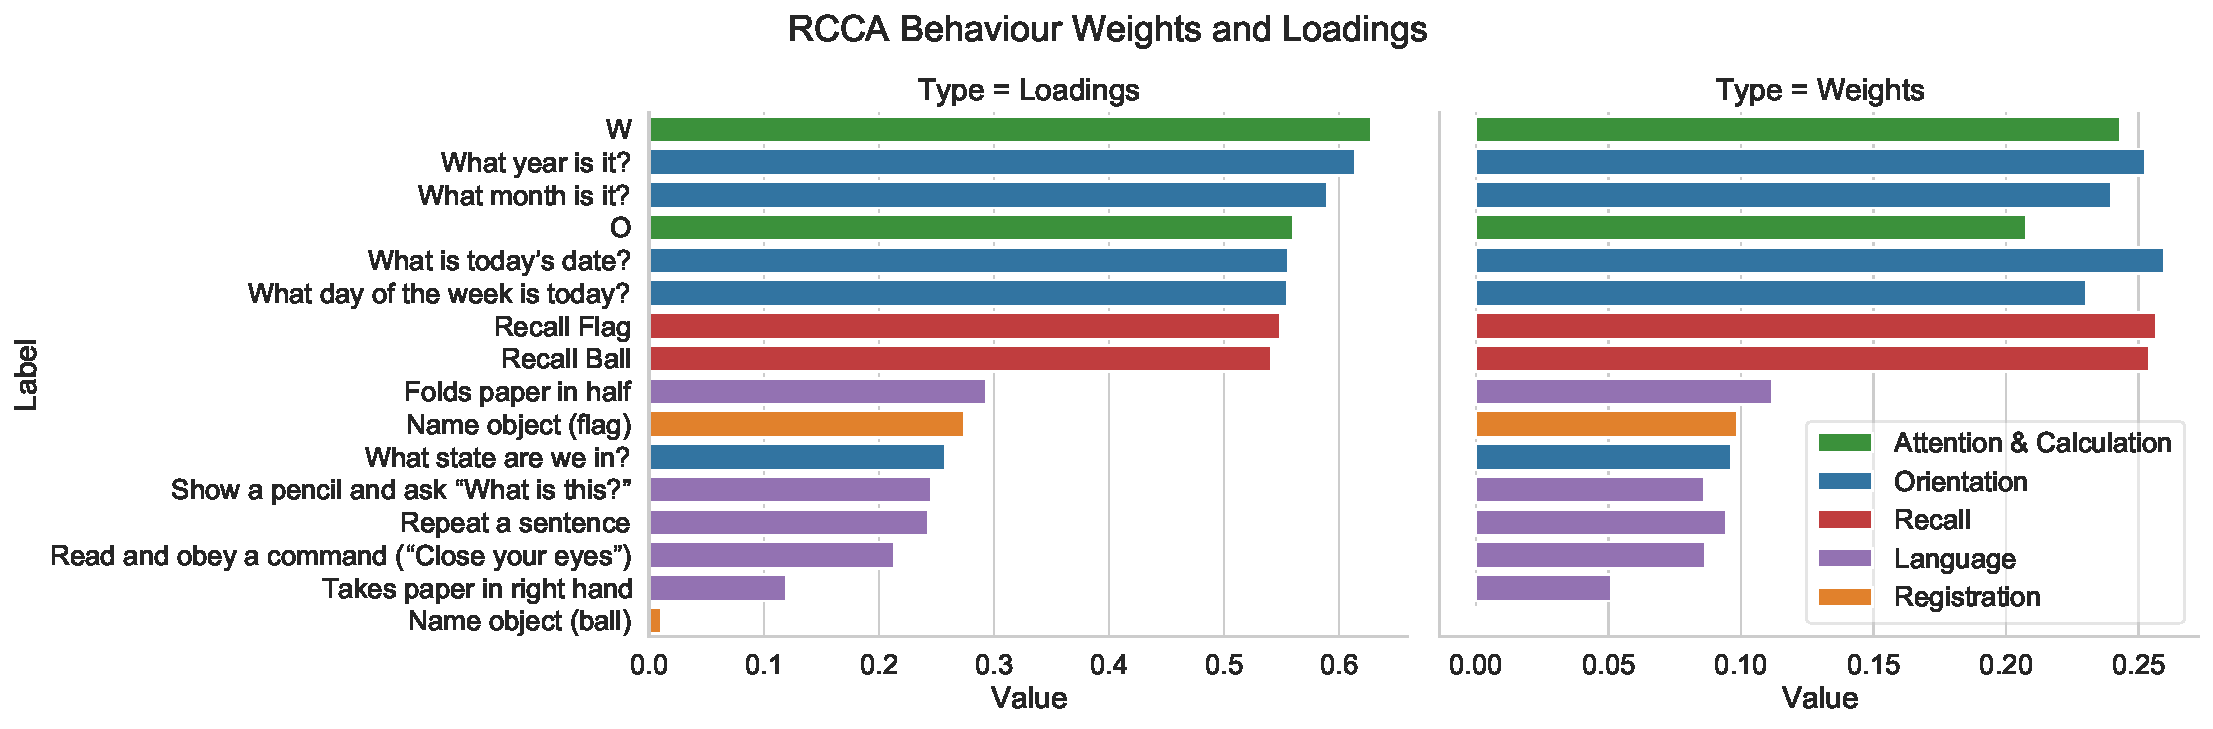
\includegraphics[width=0.8\linewidth]{figures/adni/RCCA behaviour weights and loadings}
%    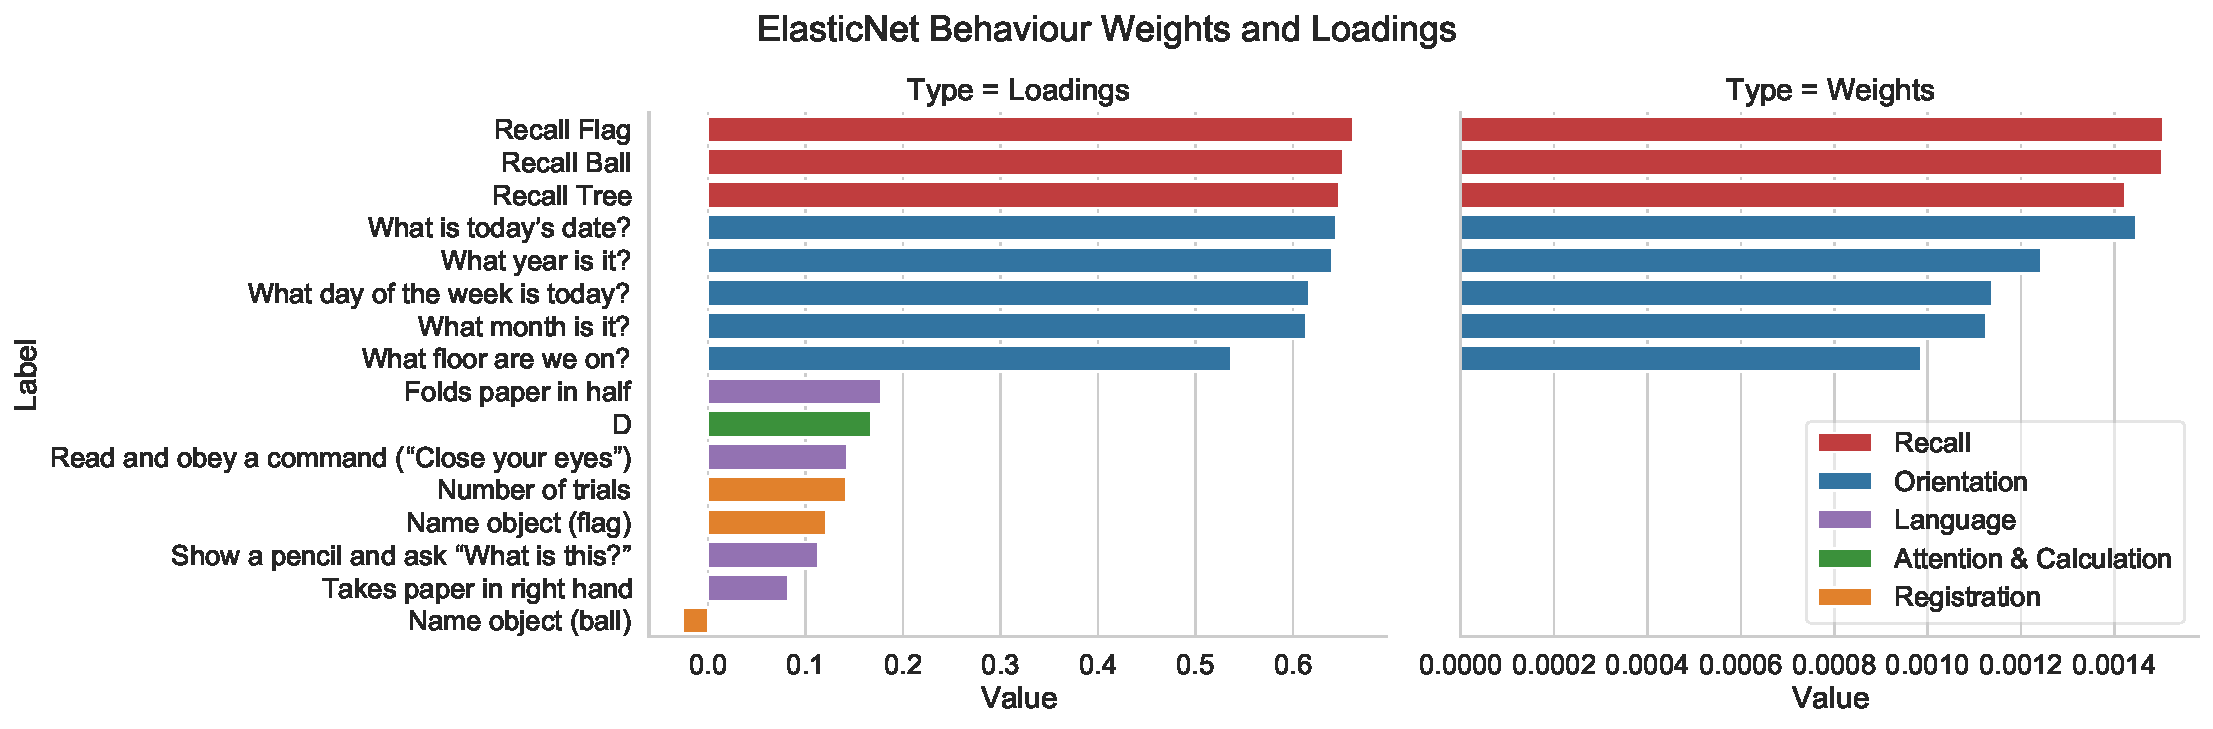
\includegraphics[width=0.8\linewidth]{figures/adni/ElasticNet behaviour weights and loadings}
%    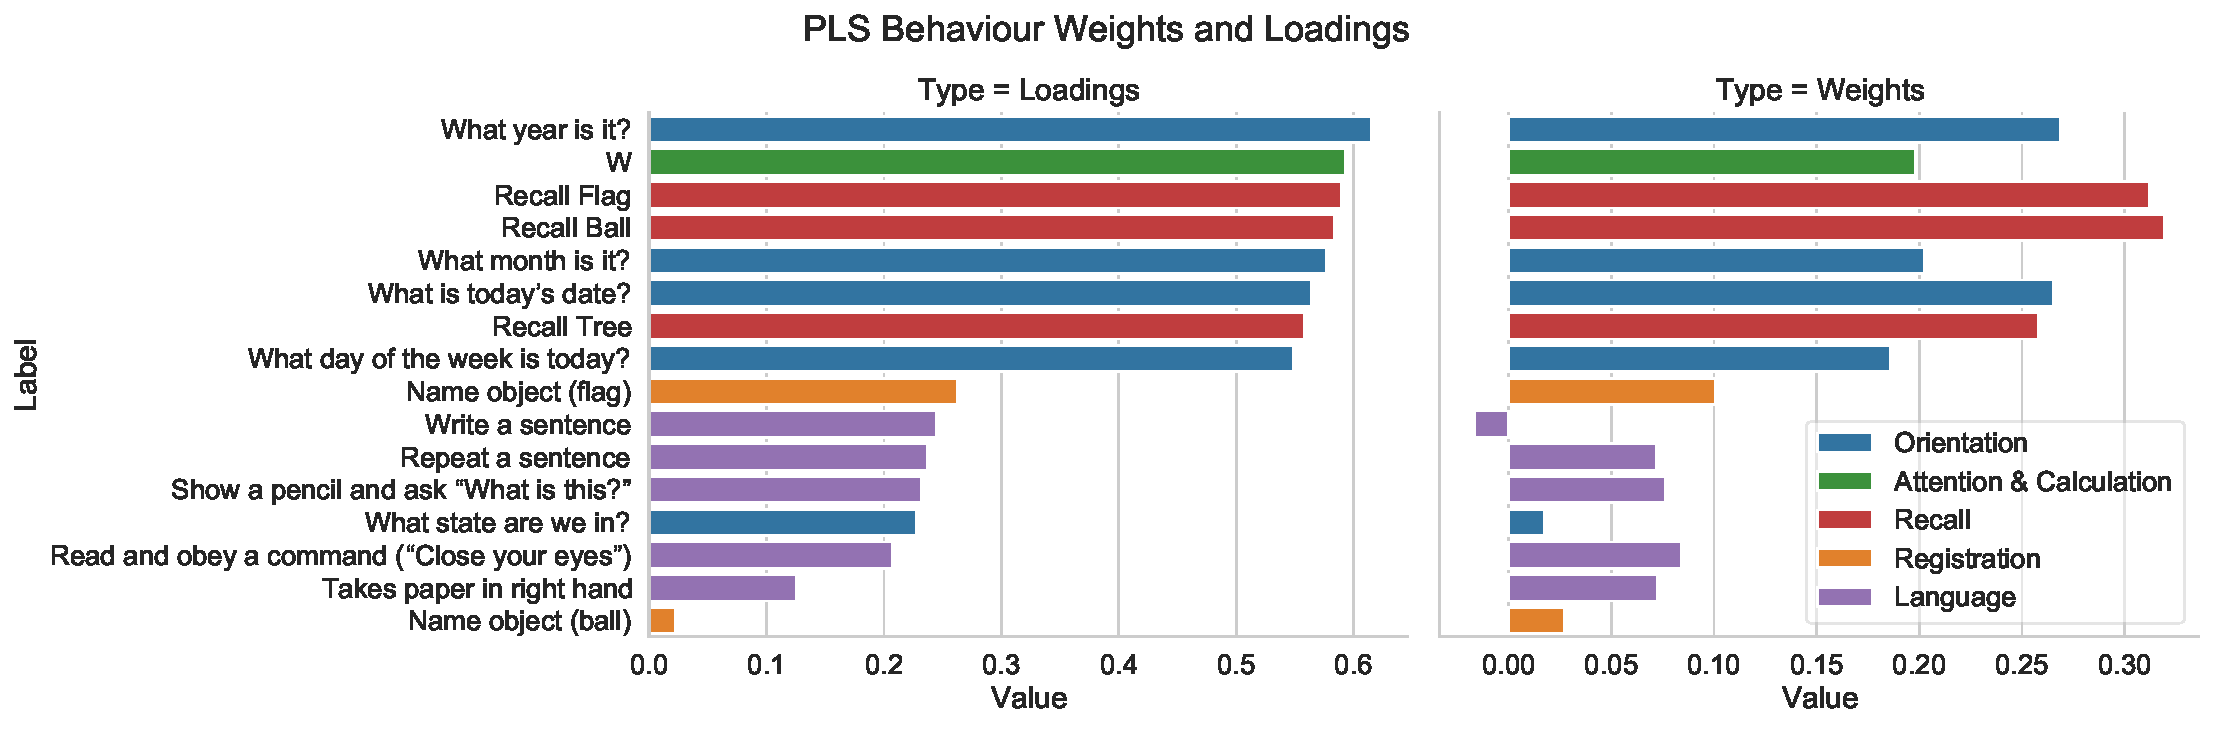
\includegraphics[width=0.8\linewidth]{figures/adni/PLS behaviour weights and loadings}
%    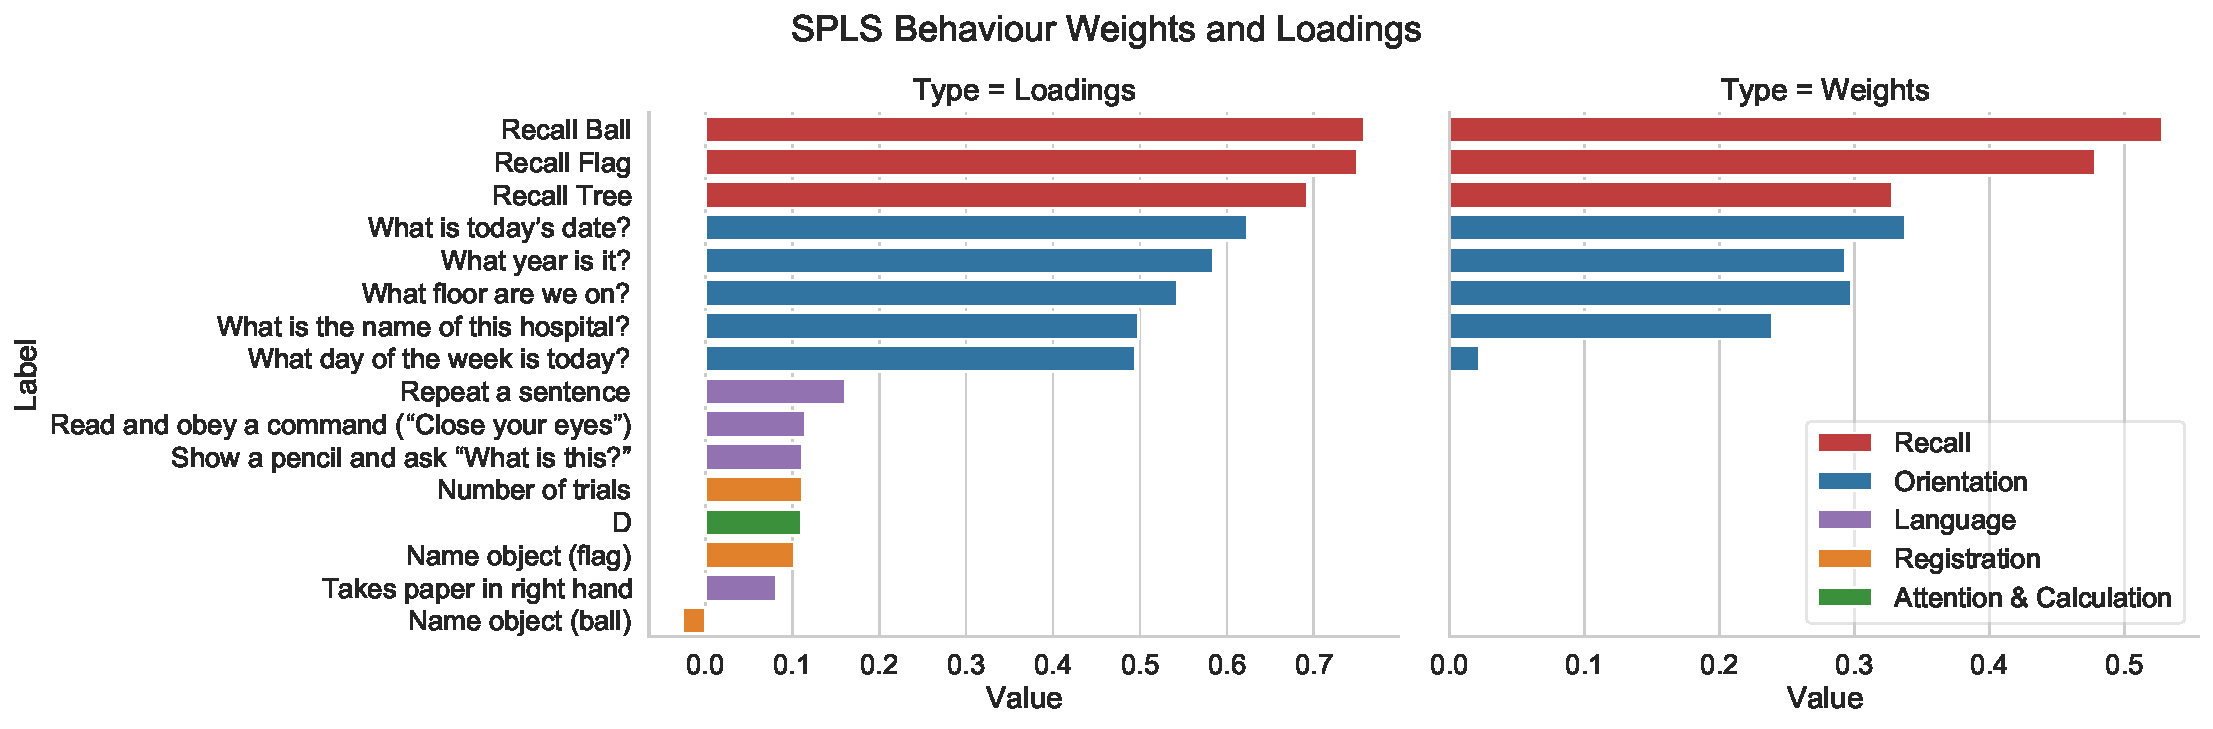
\includegraphics[width=0.8\linewidth]{figures/adni/SPLS behaviour weights and loadings}
%    \caption{Bar plots of the behaviour \gls{weights} and \gls{loadings} for each model.}
%\end{figure}

\section{Discussion}

\textcolor{red}{TO-DO: Discuss the results.}

\paragraph{Can We Construct a Regularization Functional that Imposes Sparsity on the Loadings?}
Given our observations in this chapter, a natural question to ask is whether we can construct a regularization functional that imposes sparsity on the \gls{loadings} (instead of the weights).
The answer is yes, but it is not straightforward and in the small sample setting, it is not clear that it is a good idea.
The principle would be much the same as the Lasso, but we would need to use the sample covariance matrix to define the norm:

\begin{align}
    P(W)=\|W\|_1 \\
    P(L)=\|\hat{\Sigma}U\|_1
\end{align}

Which imposes an L1 penalty on the \gls{loadings} via an L1 penalty on the \gls{weights} multiplied by the sample covariance matrix.
We could in principle apply the soft-thresholding operator to the estimated loadings.
However we would need to be careful to ensure that the sample covariance matrix is invertible in order to get back to the weights.
This is of course not guaranteed in the small sample setting.

\section{Conclusion}

In this chapter, we unified methods for generating simulated multiview data from the generative perspectives of implicit and explicit latent variable models.
We used this perspective to understand the relationship between weights and loadings in \acrshort{cca} models.
Through a mathematical argument, we showed that the \gls{loadings} are invariant to columnwise transformations of the data matrix, while the weights are not.
This is a key advantage of \gls{loadings} over weights for the interpretation of \acrshort{cca} models since it implies that weights are arbitrary and can be set to any value by scaling the data matrix or adding linear combinations of columns.
Through a series of experiments, we showed how different simulated data generation models can enhance our understanding of the properties of \acrshort{cca} and \acrshort{pls} models.